% THIS TEMPLATE IS A WORK IN PROGRESS
% Adapted from an original template by faculty at Reykjavik University, Iceland

\documentclass{scrartcl}

% Adapted from an original template by Hlyni Arnórssyni, Reykjavik University, Iceland
%
% ------------------------------ SETTINGS
\usepackage{geometry}

\geometry{
	paper=a4paper, % Paper size
	top=2.5cm, % Top margin
	bottom=2.5cm, % Bottom margin
	left=2.5cm, % Left margin
	right=2.4cm, % Right margin
	headheight=0.75cm, % Header height
	footskip=1.5cm, % Space from the bottom margin to the baseline of the footer
	headsep=0.75cm, % Space from the top margin to the baseline of the header
	%showframe, % Uncomment to show how the type block is set on the page
}

\usepackage{blindtext}
%-------------------------------- Character encoding ----------------------------
\usepackage[T1]{fontenc}
\usepackage[utf8]{inputenc}

%----------------------------- Mathematics packages from AMS ---------------

\usepackage{amsmath, amsfonts, amsthm, amssymb}
\usepackage{braket, nicefrac}

% ----------- International System of Units
\usepackage{siunitx}

%------------------------------ Lists / numbers -------------------------
\usepackage{enumitem, multicol}

%------------------------------- Figure insertions --------------
\usepackage{graphicx, float}  % Use option [H] to force the placement of a figure
\usepackage{keystroke}
\usepackage{pgfplots}\usepgfplotslibrary{units}\pgfplotsset{compat=1.16}

%------------------------------- Line Spacing --------------
\usepackage{setspace}

%------------------------------- Depth of the ToC --------------
\setcounter{tocdepth}{2}

%%%%%%%%%%%%%%%%%%%%%%%%%% Hyperlink References %%%%%%%%%%%%%%%%%%%%%%%%%%%
\usepackage{hyperref}

%--------------------% Storage Path for images %-----------------%
\graphicspath{{graphics/}{Graphics/}{./}}

%%%%%%%%%%%%%%%%%%%%%%%%%% Environments %%%%%%%%%%%%%%%%%%%%%%%%%%%
\renewenvironment{abstract}{
    \begin{center}
    \textbf{Abstract}
    \vspace{0.5cm}
    \par\itshape
    \begin{minipage}{0.8\linewidth}}{\end{minipage}
    \noindent\ignorespaces
    \end{center}
}

\newenvironment{keywords}{
    \begin{center}
    \textbf{Keywords}
    \vspace{0.5cm}
    \par
    \begin{minipage}{0.8\linewidth}}{\end{minipage}
    \noindent\ignorespaces
    \end{center}
}

\newenvironment{preface}{
    \begin{center}
    \textbf{Preface}
    \vspace{0.5cm}
    \par
    \begin{minipage}{0.8\linewidth}}{\end{minipage}
    \noindent\ignorespaces
    \end{center}
}

\newenvironment{acknowledgements}{
    \begin{center}
    \textbf{Acknowledgements}
    \vspace{0.5cm}
    \par
    \begin{minipage}{0.8\linewidth}}{\end{minipage}
    \noindent\ignorespaces
    \end{center}
}
\usepackage{listings}
\usepackage{minted}
\usepackage[colorlinks,linkcolor=red]{hyperref}
\hypersetup{
colorlinks=true,
linkcolor=black
}
% \usepackage[style=numeric-comp,sorting=none,url=false]{biblatex}



\begin{document}
%Title of the report, name of coworkers and dates (of experiment and of report).
\begin{titlepage}
	\centering
	\includegraphics[width=0.6\textwidth]{Graphics/DKU Logo_clean.png}\par
	\vspace{2cm}
	%%%% COMMENT OUT irrelevant lines among the 3 below
	
	{\scshape\LARGE Data Science \par}      %if you're a DS major
	\vspace{1cm}
	{\scshape\Large STATS210 Final Project Report - Spring 2022\par}
	%{\large \today\par}
	\vfill
	
	%%%% PROJECT TITLE
	{\huge\bfseries The Red Envelope Problem\par}
	\vfill
	
	%%%% AUTHOR(S)
	{\Large\itshape Jingheng Huan,\\Xuanang Zhou,\\Yueqian Lin,\\Zhixian Zhang}\par
	\vspace{2cm}

	\vfill
	supervised by\par
	%%%% SUPERVISOR(S)
	Prof. Pingqiang Zhou \& Bohuan Li


	\vfill
% Bottom of the page
\end{titlepage}

% \newpage

% \begin{preface}
    
% \end{preface}

% \vspace{1cm}

% \begin{acknowledgements}
% The authors thank the support of the course instructor and teaching assistant.
% \end{acknowledgements}

\newpage


\begin{abstract}
	    With the widespread use of mobile phone, the random amount red envelope grabbing is becoming more and more popular. Probability is a discipline that studies the statistical laws of random phenomena, and by studying the probability distribution of red envelope, this paper tries to explain the effect of the order of grabbing red envelope on the amount of money. In our experiment, we used Python to do simulation and draw plots. We construct a distribution mechanism based on experimental data and relevant analysis. We also compare our mechanism with experimental data in different aspects. Based on the results, several suggestions are made to people with different goals. Additional analysis is carried out for the luckiest people solitaire game.
\end{abstract}
\vspace{1cm}

\begin{keywords}
\centering
        \textbf{Red envelope; Statistics; Monte-Carlo simulation; Data visualization; Duke Kunshan}
\end{keywords}

\newpage



\doublespacing
\tableofcontents
\singlespacing

\newpage

\doublespacing

\section{Introduction}
\label{sec1}
Giving red envelopes is a traditional custom at the beginning of the Chinese New Year. A red envelope is a type of money bag, also known as "lucky money". People believe that those who receive red envelopes will have good luck in the coming year.
However, in recent years, a  function on WeChat called “random amount red envelope” has been very popular. This kind of envelope is more popular than the normal red envelope because it is full of uncertainties and comparisons with other money takers. People who receive little money from random red envelopes always complain the fairness of this kind of red envelope. Nevertheless, we believe that the reason people receive fewer random red envelopes is not bad luck, but a specific algorithm and distribution behind the server.

In this project, our team try to apply Monte-Carlo simulation to find out the algorithm and mathematical model of WeChat red envelopes. We  firstly experiment on WeChat by sending and grabbing 120 times random red envelopes and then record the results. After the experiment, the results are analyzed and displayed through using data visualization techniques. Next, based on some key findings and mathematical knowledge, our team combines some existing literature and k-s test to design the distribution mechanism of random amount red envelope. After that, we use Python to implement the model. After validating our model by comparing the simulated distribution with the actual results, we use this simulation model to obtain more findings of WeChat red envelopes patterns and then provide suggestions for the users who want to grab more money from WeChat red envelopes. We also perform some additional analysis on luckiest people in one envelope and red envelope solitaire.

\section{Experiment}\label{sec2}
\subsection{Experiment Process}
\label{sec2.1}
We gathered 8 people in a WeChat group and each person sent 15 red envelops, for a total of 120 red envelopes. The money in each envelope was 10 yuan and was randomly divided into 8 pieces. After all 8 people had grabbed all the envelopes, we recorded the corresponding order of grabbing money and the number of trials for each of the 8 people. Based on the experiment results, we use Python to analyze the patterns and design our simulation model.

\subsection{Experiment Results}
\label{sec2.2}
After recording and plotting the results, in Figure \ref{Mess}, from the density of the lines we can see that there are more chances to grab a greater amount of money if we grab the red pocket later. In Figure \ref{mean_var_exp}, we can see that with the order of pick increases, the mean of the money taken by each order does not deviate among orders. However, the variance varies among different orders. Theoretically, the variance of money will increase as the order increase. In our experiment, the variance does not strictly follow what is derived in mathematical analysis in Section \ref{sec3.1}. The reason is that our sample space is not large enough. In Section \ref{sec4.2}, it is shown that when the sample space is large enough, the mean and variance follow the distribution derived in Section \ref{sec3.1}. In Figure \ref{PriceDistribution_1}, we observe the price distribution in each pick and plot the histogram. We can see that in the later picks (4-8), not only it is more likely to grab a huge amount, but also there are more chance to grab just a tiny amount. In the early picks (1-4), although there are seldom big picks, the risk of grabbing tiny amount of money is also lower than the later picks. Based on the observations above, we make the hypothesis that the mean value of different picks remain constant, but the variance of different picks increase as the order of pick increase. Namely, the early picks have consistency while the later picks have both higher profit and higher risk. Figure \ref{PriceDistribution_2} shows the price distribution of different participants. It reveals that all of the eight participants got similar distribution over price, and the peak of the distribution always falls between $0 - 2.5$ yuan, in which the mean money of each participant also falls into. It means that no one has a privilege over another. Our experiment is fair and the results are reliable. 

\begin{figure}[H]
	\begin{center}
		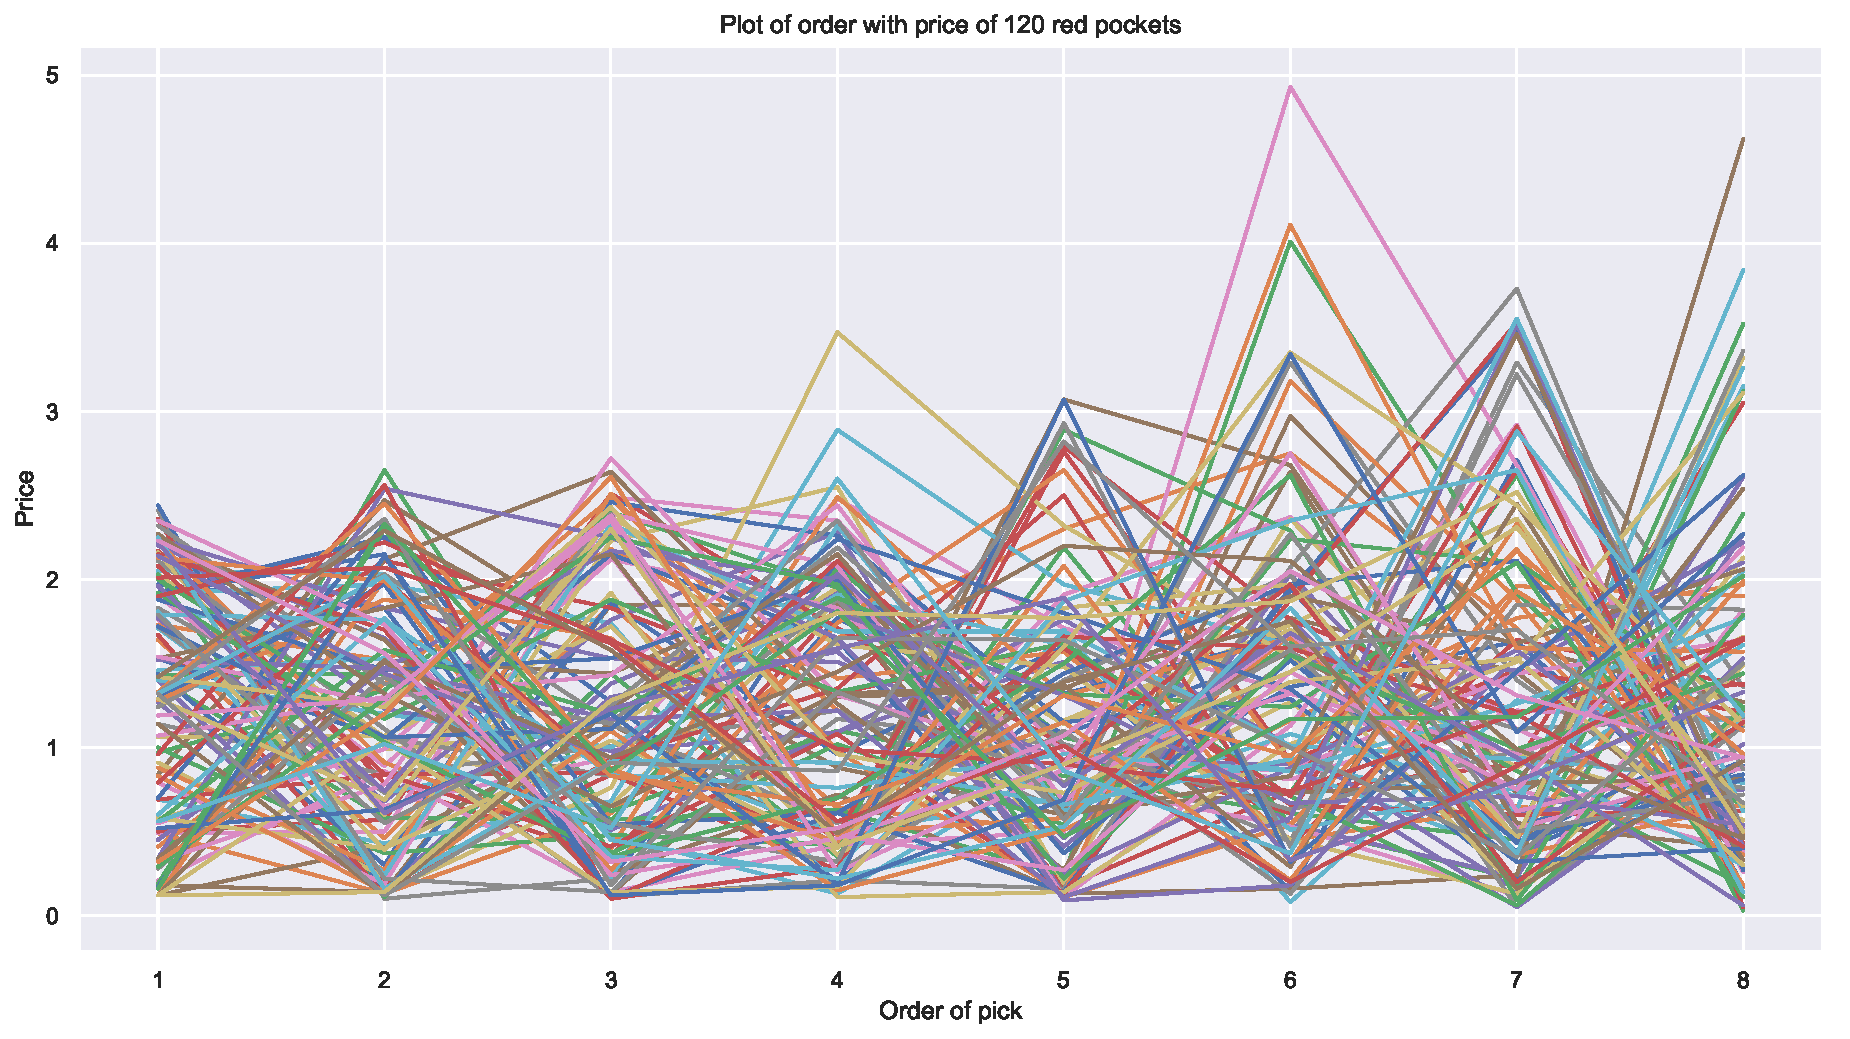
\includegraphics[width=15cm]{pic6.pdf}
	\end{center}
	\caption{Relation between Order and Price in 120 Red Envelopes}
	\label{Mess}
\end{figure}

\begin{figure}[H]
\centering    
\subfigure{
\label{mean_exp}
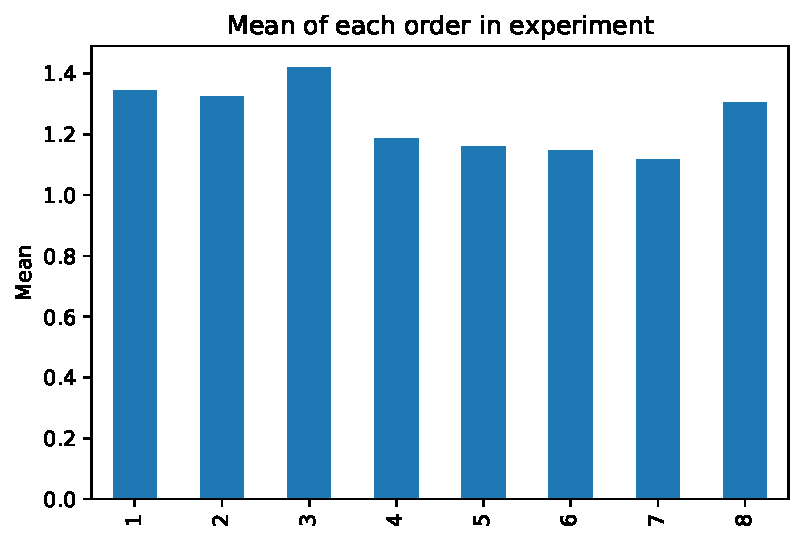
\includegraphics[width=0.4\columnwidth]{mean_experiment.pdf}  
}     
\subfigure{ 
\label{var_exp}     
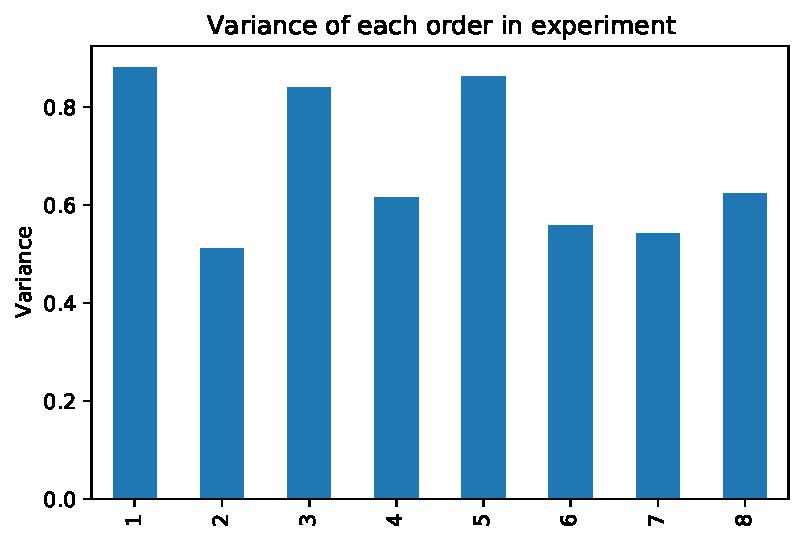
\includegraphics[width=0.4\columnwidth]{variance_experiment.pdf}
}    
\caption{ Mean and Variance of Each Order In the Experiment}     
\label{mean_var_exp} 
\end{figure}

\begin{figure}[H]
	\begin{center}
		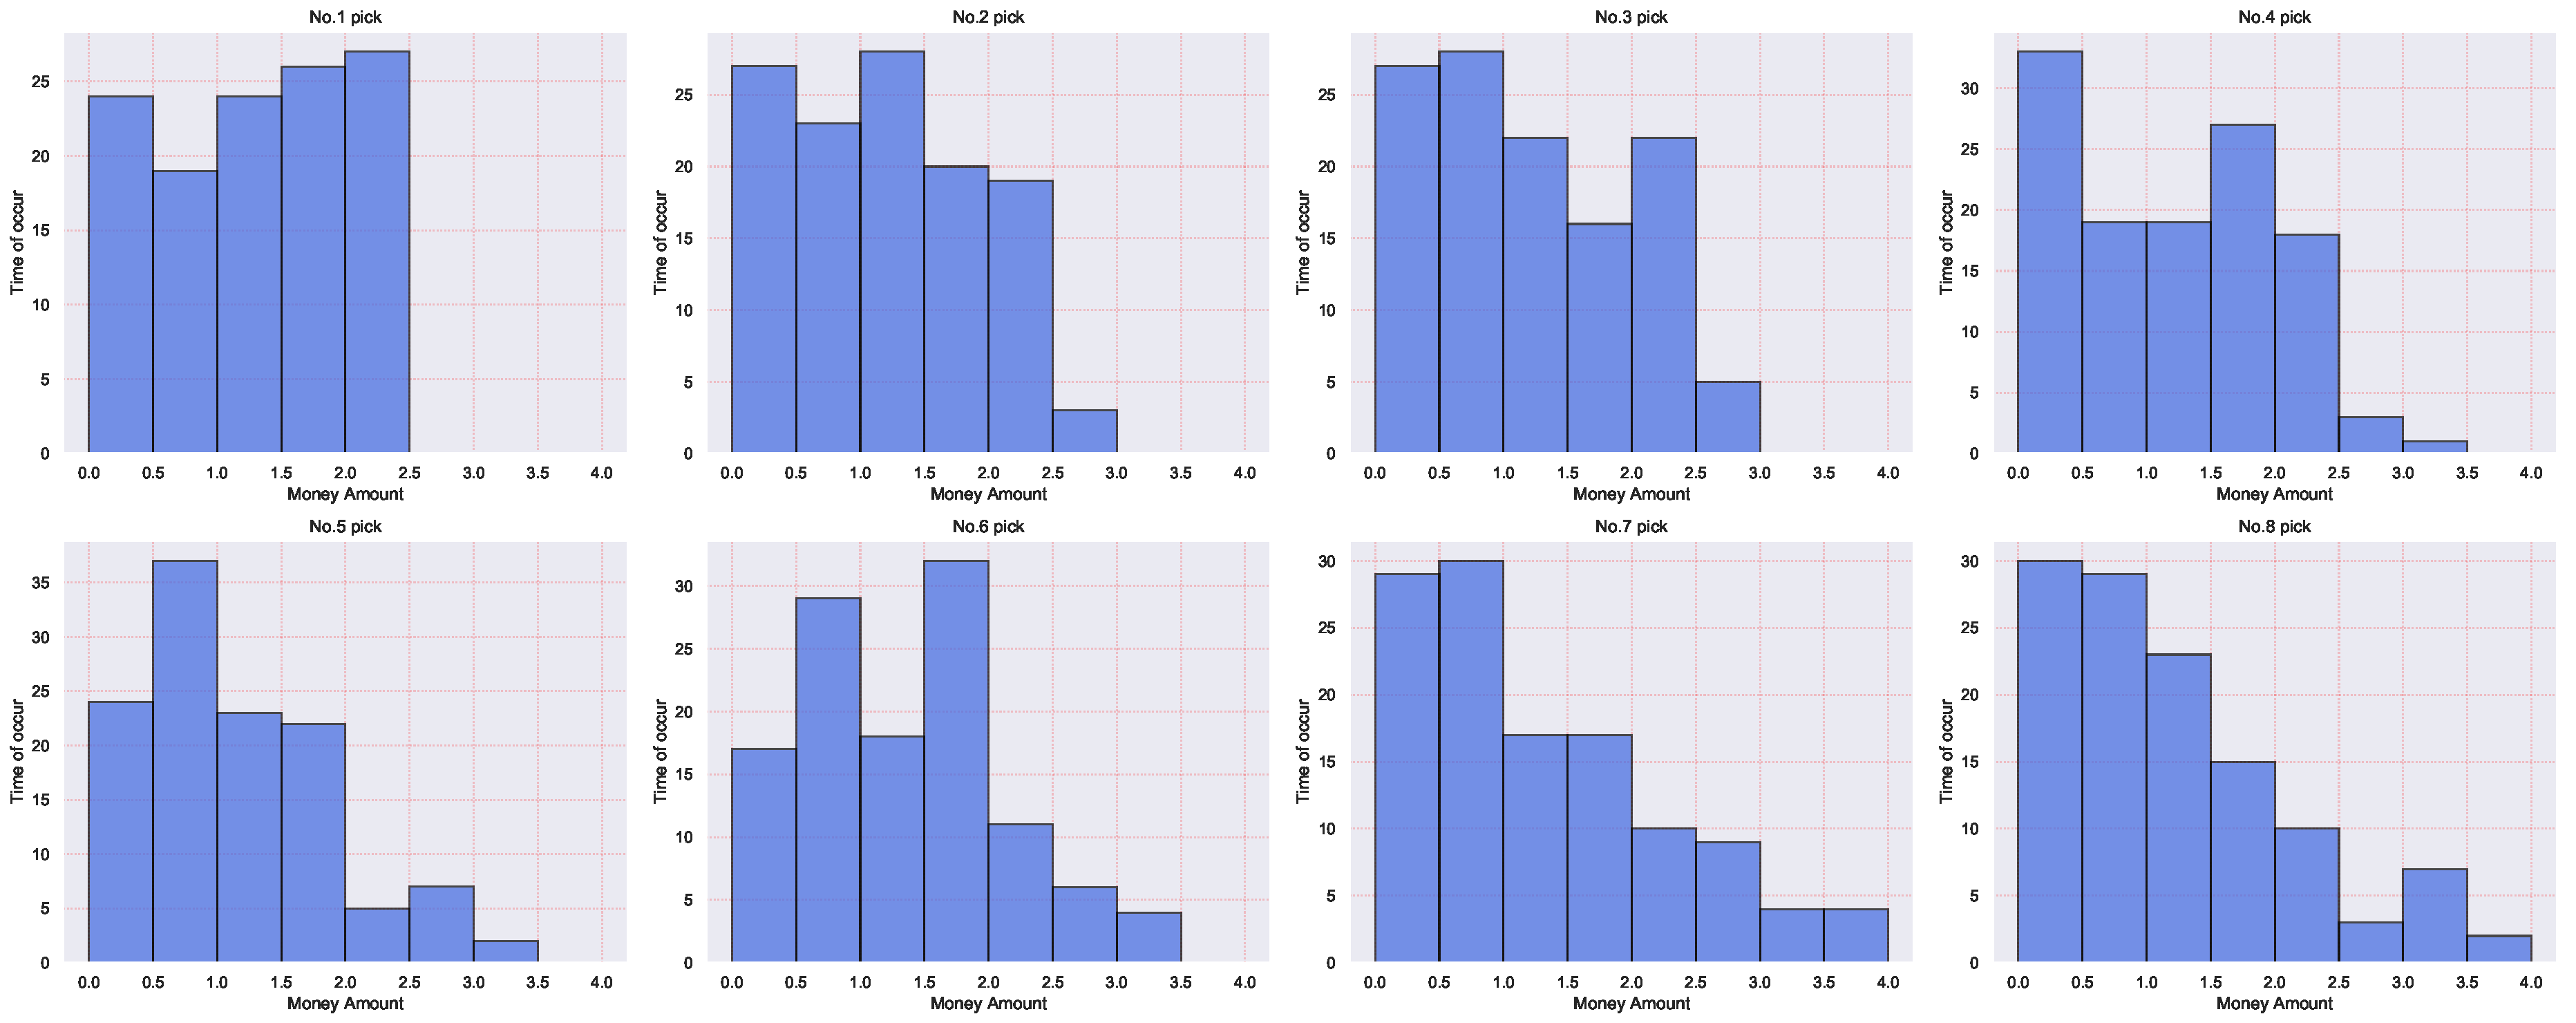
\includegraphics[width=15cm]{pic10.pdf}
	\end{center}
	\caption{Money Distribution of Different Picks}
	\label{PriceDistribution_1}
\end{figure}

\begin{figure}[H]
	\begin{center}
		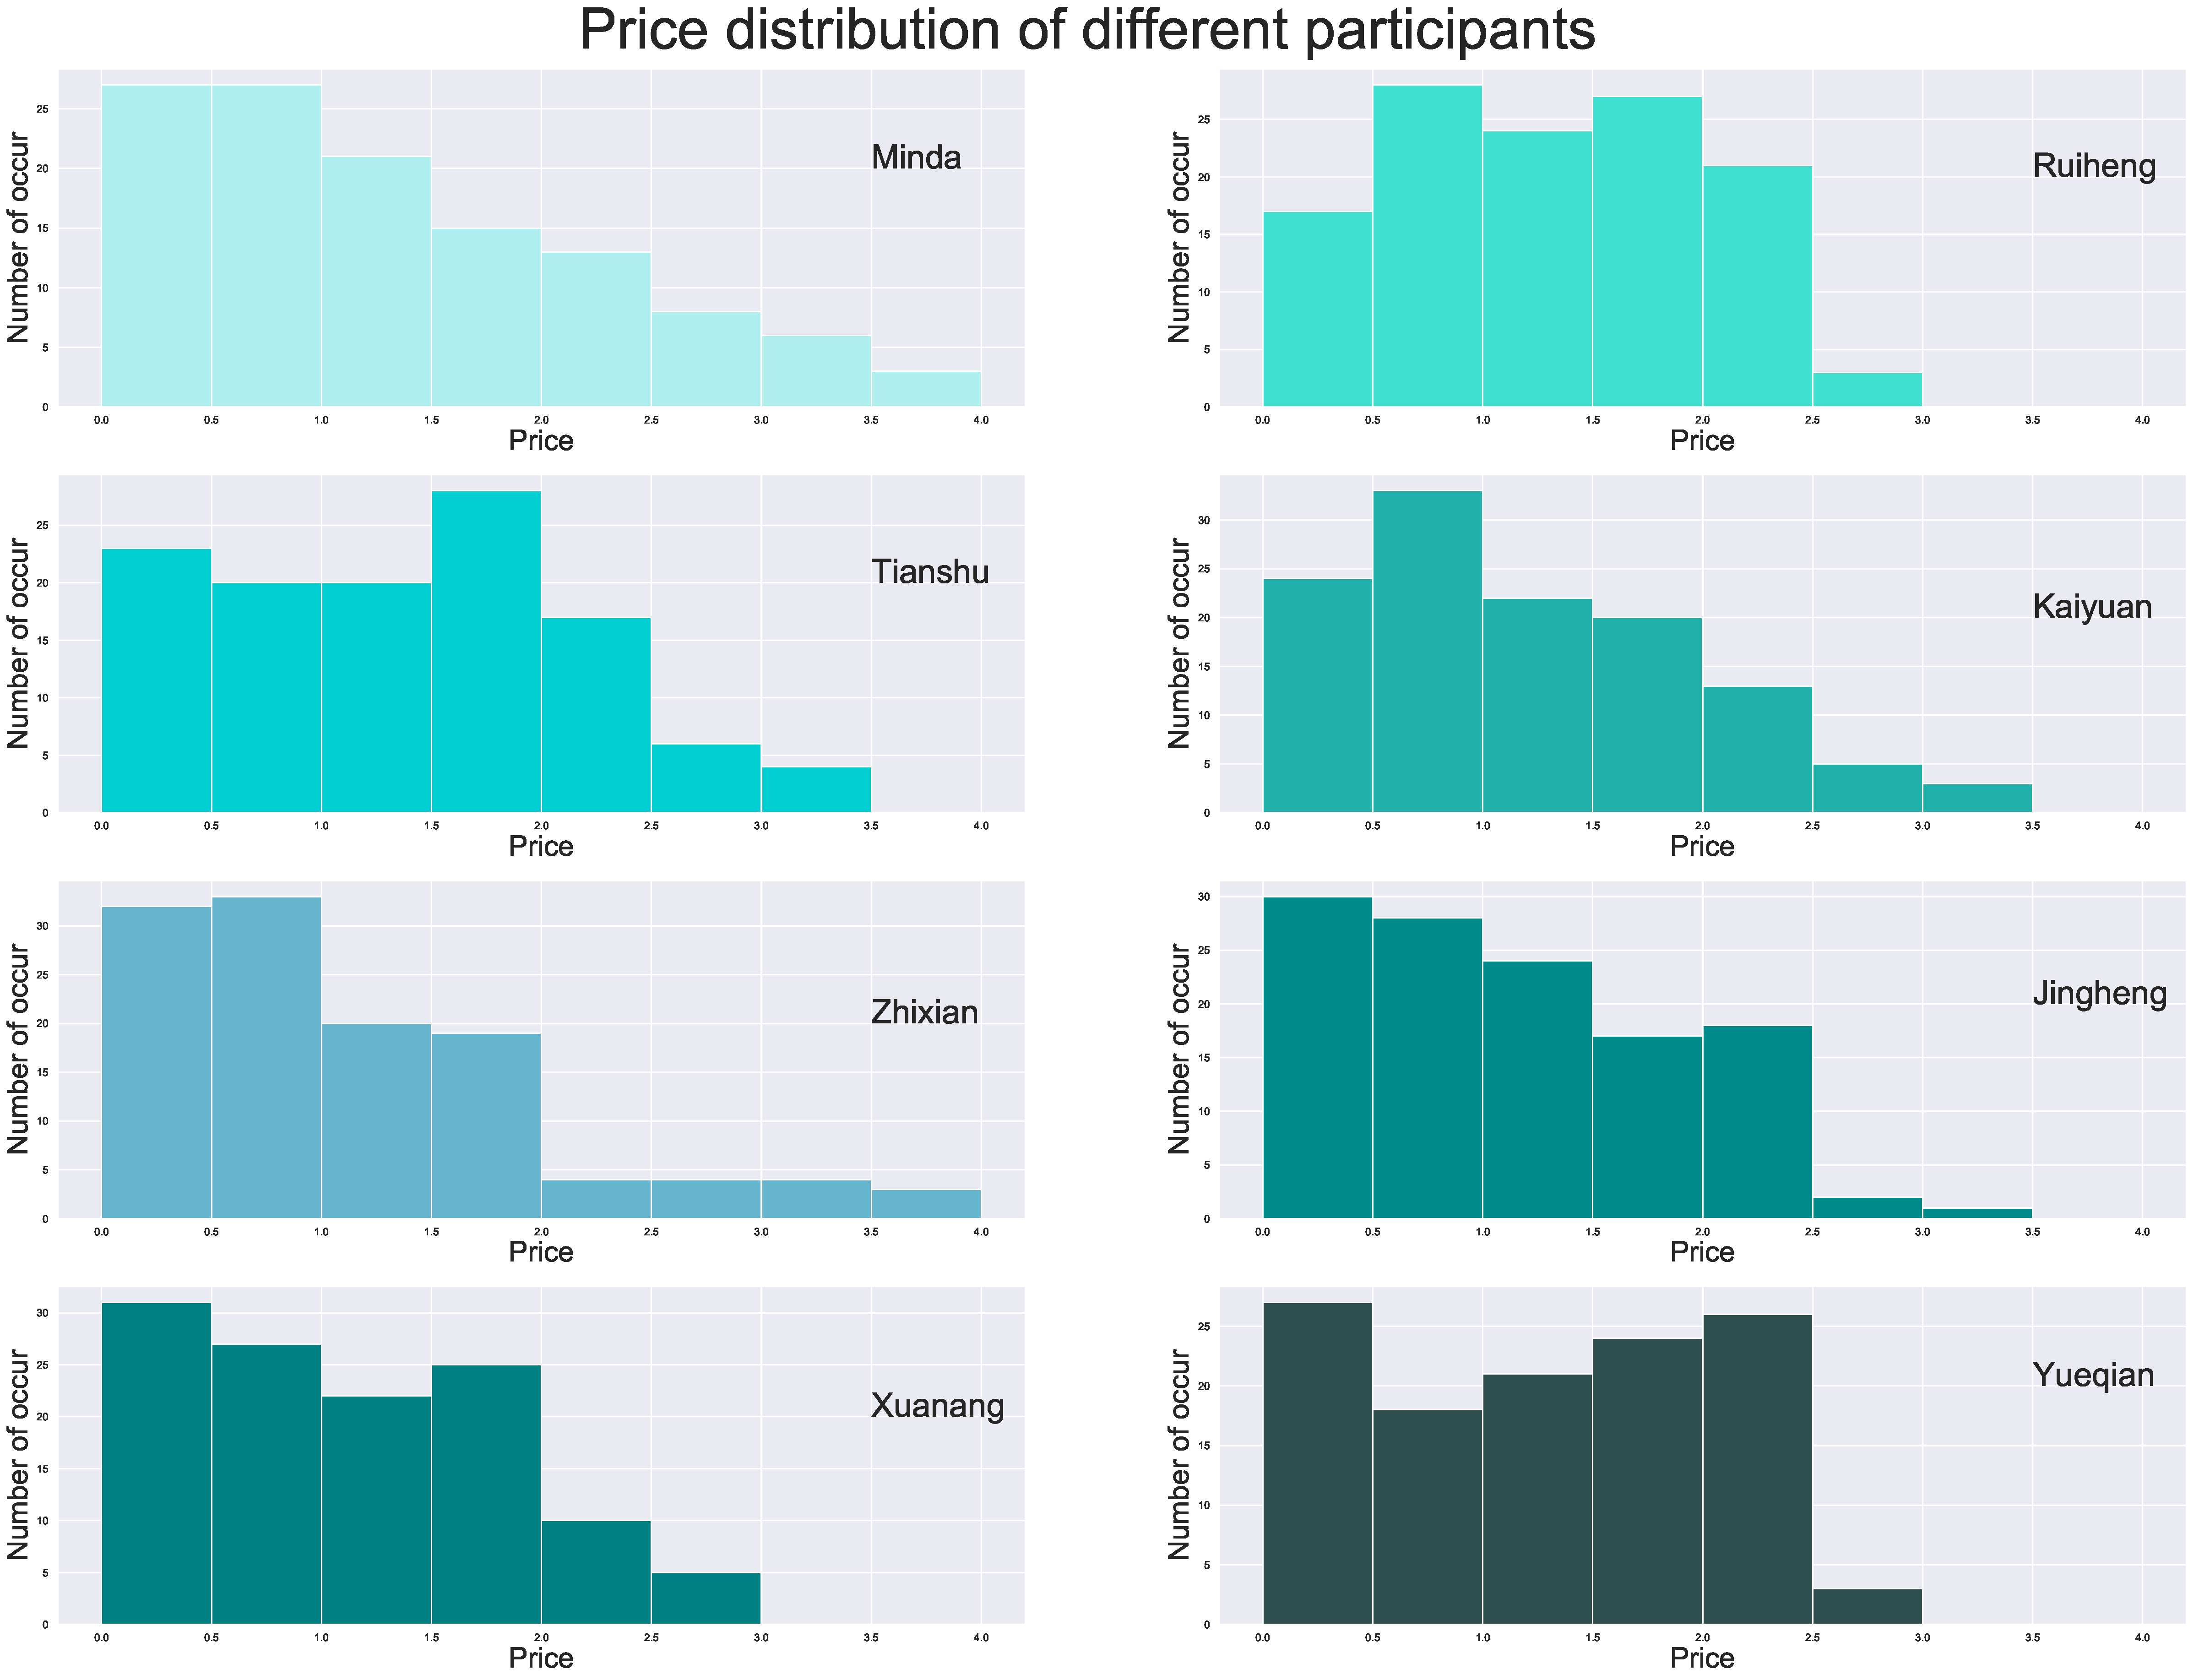
\includegraphics[width=16cm]{pic11.pdf}
	\end{center}
	\caption{Price Distribution of Different Participants}
	\label{PriceDistribution_2}
\end{figure}

\section{Simulation by Programming}


\subsection{Distribution Mechanism}\label{sec3.2}
Based on the visualizations and  analysis of experimental data before, we can give an assumption of the distribution mechanism. The distribution mechanism can be divided into two parts: what probability distribution does every grab fit and what is the range of such distribution.
\subsubsection{Probability Distribution Type}
To the first part, we can use Kolmogorov-Smirnov test (simplified as k-s test) to compare the experimental distribution $f(x)$ and theoretical distribution $g(x)$ \cite{bergerKolmogorovSmirnovTest2014}. Through the visualization of experimental data before, it is not difficult to find that the amount of money of each pick is fairly evenly distributed over a specific range.  As a result, we assume that the data points satisfy the uniformly distribution. Thus, to verify it, we compare the experimental distribution $f(x)$ and uniform distribution $g(x)$. This process is a hypothesis test and
\begin{itemize}
\item $H_0$: The experimental data samples conform to uniform distribution.
\item $H_1$: The experimental data sample does not conform to uniform distribution.
\end{itemize}\par
Whether we accept or refuse $H_0$ is based on the value of D. Also, we use sample size $n$ and significant level $a$ to find $D(n,a)$ from critical values table. If $D < D(n,a)$, we accept the hypothesis $H_0$. 
$$D=\max|f(x)-g(x)| $$\par
This is the theorem of k-s test. When we perform k-s test with python, we should decide if we accept or refuse the hypothesis based on p-value.If $\text{p-value} > 0.05$, we accept the $H_0$. The visualization of the comparison of $f(x)$ and $g(x)$ for each order is shown below.
\begin{figure}[H]
	\begin{center}
		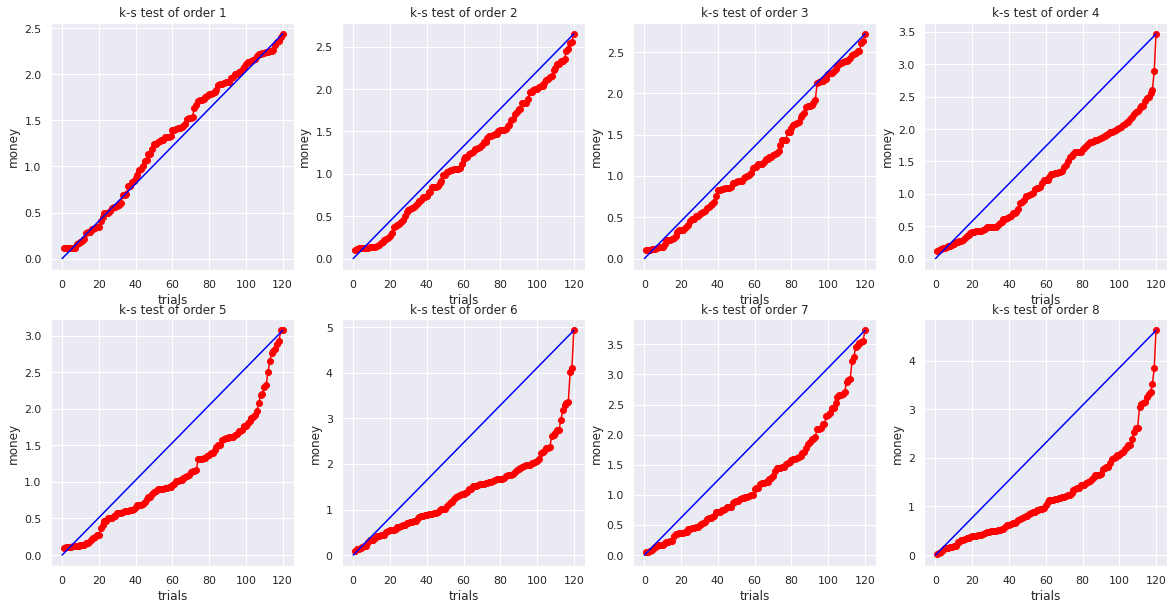
\includegraphics[width=15cm]{下载.png}
	\end{center}
	\caption{k-s test fitting for each order of pic}
	\label{code}
\end{figure}
From the comparison visualization, we know that the p-value of the first order and the second order of pick $>0.05$, thus accepting $H_0$. While for the rest order of pick, from the picture we can find that it does not look like a uniform distribution because $D$ is larger than $D(n,a)$. However, it is also obvious that several data points are much larger than the rest data points, which is the most part of data set. If we exclude these several extreme points, the distributions of these order of picks are also uniform. The visualization results also show that that the variation of data set becomes larger as the order increasing, which will be proved in detail later.
\subsubsection{Distribution Parameter and Result}
To the second part of distribution design, which asks us to estimate the parameter of distribution, our team apply Maximum Likelihood Estimation to get the boundary of uniform distribution (Given distribution calculate parameter).
The likelihood function can be written as
$$\prod \limits_{i=1}^n f(x_{i};a,b) = \frac{1}{(b-a)^n}$$
\indent and the log-likelihood function can be written as 
$$\log \prod \limits_{i=1}^n f(x_{i};a,b) = \log \frac{1}{(b-a)^n}=-n\log(b-a)$$\par
To Find the values for $a$ and $b$ that maximize the log-likelihood function, we can take the derivative of the log-likelihood function with respect to $a$ and $b$. The result is $n/(b-a)$ and $-n/(b-a)$. Since the derivative with respect to $a$ is monotonically increasing. As a result, the MLE for a would be the minimum value of each order's data set.  Since the derivative with respect to $b$ is monotonically decreasing. As a result, the MLE for $b$ would be the maximum value of each order's data set. In other words, $a$ and $b$ are separately the minimum value and the maximum value of a data set.

Now, we have determined the distribution type and distribution parameter. We need to use this to figure out how money is really distributed in random amount red envelope. To achieve it, we also need to combine the hint that the amount of money I get is generated based on the remaining gross money and remaining number of money takers at the time I send “grab” command. It is naturally for us to consider the mean of remaining money. To the first pick, no data we collect is over 2.5, which is the twice of the mean of the remaining money. Based on the same rule, we calculate the range for the second order (twice of the mean of the rest) and find that no data of the second order is over it. In addition, for each order there exists someone taking a very small amount of money, but all have at least 0.01 yuan. Therefore, combining the rigorous analysis and related literature, our team assumes that the real distribution mechanism is

\centerline{\textbf{The amount of money each one can grab is uniformly }}
\centerline{\textbf{distributed from 0.01 yuan to twice the mean of the rest money.}}
\subsection{Mathematical Analysis on Expectation and Variance Based on Our Mechanism}\label{sec3.1}
From the description of Task 3, we know that WeChat handles the high frequency of millions of red envelopes being grabbed around the world by using an online algorithm that only generates the amount of money when you actually send the "grab" command. In this case, we should apply the distribution mechanism we derive in the section 3.1.2. We denote the total number of red pockets as  $n$, the total amount of money as  $S$ \cite{bidaothuWoGeiZiJiFaLiao2YiGeHongBaoCaiFaXianXianQiangHeHouQiangChaiJuZheMeDaBiLiBiLi}. $X_{i}$  represents the money taken by  the $i^{t h}$  taker.  $S_{i}$  represents the sum of money after  $i^{\text{th}}$  taker opens the red pocket. We definite  $S_{0}=0$, $X_{0}=0$ . We know that
$$\left\{\begin{array}{c}
X_{1} \sim \text{Uniform}\left(0.01,\frac{2S}{n}\right) \\
X_{k+1} \sim \text { Uniform }\left(0.01,2 \frac{S-S_{k}}{n-k}\right) \\
S_{k}=X_{1}+X_{2}+X_{3} \ldots+X_{k}
\end{array}\right.$$\par
We want to prove that
$E\left[X_{1}\right]=E\left[X_{2}\right]=\cdots=E\left[X_{n}\right], \operatorname{Var}\left[X_{1}\right]<\operatorname{Var}\left[X_{2}\right]<\cdots<\operatorname{Var}\left[X_{n}\right]$.

We know that the money for the last two people have the same distribution.

$$\mathrm{E}\left[S_{k}^{m}\right]=\int_{-\infty}^{\infty} x^{m} \cdot f_{S_{k}}(x) d x$$

where  $f_{S_{k}}(x)=f_{S_{k} \mid S_{k-1}}(x \mid y) \cdot f_{S_{k-1}}(y) d y $

$$f_{S_{k} \mid s_{k-1}}(x \mid y)=\mathrm{P}\left(S_{k-1}=y, S_{k}=x\right)=\frac{n-k+1}{2(s-y)}$$

when  $x\in\left[y, y+\frac{2(s-y)}{n-k+1}\right] $\par
Thus,

$$\begin{array}{l}\mathrm{E}\left[S_{k}^{m}\right]
=\int x^{m} \cdot\left(f_{S_{k} \mid S_{k-1}}(x \mid y) \cdot f_{S_{k-1}}(y) d y\right) d x \\
\quad=\int x^{m} \cdot\left(\int \frac{n-k+1}{2(s-y)} \cdot I(x) \cdot f_{S_{k-1}}(y) d y\right) d x \\
\quad=\int \frac{n-k+1}{2(s-y)} \cdot f_{S_{k-1}}(y)\left(\int x^{m} \cdot I(x) d x\right) d y
\end{array}$$

where  $\mathrm{I}(\mathrm{x})=1  \text { when }  x \in\left[y, y+\frac{2(s-y)}{n-k+1}\right]\text{, } \mathrm{I}(\mathrm{x})=0$ otherwise.\par
When $\mathrm{m} =1$,
$\mathrm{E}\left[S_{k}\right]=\int\left(\frac{s}{n-k+1}+\frac{n-k}{n-k+1} y\right) f_{S_{k-1}}(y) d y=\frac{s}{n-k+1}+\frac{n-k}{n-k+1} \mathrm{E}\left[S_{k-1}\right]$.

Since the initial condition:  $\mathrm{E}\left[S_{1}\right]=\frac{S}{n} $ through recursion we get the equation that

$$\begin{array}{c}
\frac{S-\mathrm{E}\left[S_{k}\right]}{n-k}=\frac{S-\mathrm{E}\left[S_{k-1}\right]}{n-(k-1)} 
\Rightarrow \mathrm{E}\left[S_{k}\right]=\frac{k S}{n} 
\Rightarrow \mathrm{E}\left[X_{k}\right]=\mathrm{E}\left[S_{k}-S_{k-1}\right]=\frac{s}{n}
\end{array}$$

It shows that for each  $\mathrm{k}<=\mathrm{n}$, $\mathrm{E}\left[X_{k}\right]$  is constant and equal to  $\frac{S}{n}$.

Next, we need to prove that 
$\operatorname{Var}\left[X_{1}\right]<\operatorname{Var}\left[X_{2}\right]<\cdots<\operatorname{Var}\left[X_{n-1}\right]\leq\operatorname{Var}\left[X_{n}\right] $. Since  $\operatorname{Var}[X]=E\left[X^{2}\right]-(E[X])^{2}$, we only need to compare  $E\left[X_{k}^{2}\right]$ . First we calculate  $E\left[S_{k}^{2}\right]$, then we find the relationship between  $E\left[X_{k}^{2}\right]$  and  $E\left[S_{k}^{2}\right]$.

When  \mathrm{m}=2, $E\left[S_{k}^{2}\right]=\int \frac{1}{6} \cdot f_{S_{k-1}}(y)\left(\frac{12(S-y) y}{n-k+1}+6 y^{2}+\frac{8(S-y)^{2}}{(n-k+1)^{2}}\right) d y .$  Simplify it and we get:
\begin{equation}
\begin{aligned}
   3(n-k+1) E\left[S_{k}^{2}\right] =\qquad\qquad\qquad\qquad\qquad\qquad\qquad\qquad\qquad\qquad\qquad\qquad\qquad\qquad\qquad
\\
 \frac{6(k-1)(n-k+1)-8(k-1)+4 n}{n} S^{2}+\left(3(n-k+1)^{2}+4-6(n-k+1)\right) E\left[{ }S_{_{k-1}}^{2}\right]  
\end{aligned}
\label{eq1} 
\end{equation}


Similarly, we can derive the expectation for  $X_{k}^{m} $ by
$\par
E\left[X_{k}^{m}\right] = \int x^{m} f_{x_{k}}(x) d x = \int x^{m}\left(\int f_{x_{k} \mid S_{k-1}}(x \mid y) f_{S_{k-1}}(y)\right) d x = \int x^{m}\left(\int \frac{n-k+1}{2(S-y)} I(x) f_{S_{k-1}}(y) d y\right) d x$

$$
\begin{array}{l} = \int \frac{n-k+1}{2(s-y)} f_{S_{k-1}}(y)\left(\int_{0}^{\frac{2 s-2 y}{n-k+1}} x^{m} d x\right) d y \\ = \int \frac{2^{m}(S-y)^{m}}{(k+1)(n-k+1)^{m}} f_{S_{k-1}}(y) d y
\end{array}$$

where $I  (x) = 1$  when  $x \in\left[0, \frac{2(s-y)}{n-k+1}\right]$, $I(x) = 0$  otherwise.\par Let  $m = 2$ , and simplify the equation we get:
\begin{equation}
    3(n-k+1)^{2} E\left[X_{k}^{2}\right] = \frac{4(n-2 k+2)}{n} S^{2}+4 E\left[S_{k-1}^{2}\right]\label{eq2}
\end{equation}


We plug equation \eqref{eq2} into equation \eqref{eq1} and get:
$$
\begin{array}{c}
3(n-k)^{2} E\left[X_{k+1}^{2}\right] = \left(3(n-k)^{2}+1\right) E\left[X_{k}^{2}\right] 
\Rightarrow E\left[X_{k+1}^{2}\right] = \frac{4 S^{2}}{3 n^{2}} \prod_{i = 1}^{k}\left(1+\frac{1}{3(n-k)^{2}}\right)
\end{array}$$
\par
As $k$ increases, $E\left[X_{k+1}^{2}\right]$  increases. Finally we get:

$$\operatorname{Var} X_{1}<\operatorname{Var} X_{2}<\ldots<\operatorname{Var} X_{n-1} = \operatorname{Var} X_{n}$$
Then we draw the conclusion that the expectation is not related with the order and keep constant while the variance is increasing during the process of grabbing.


\subsection{Code Implementation}\label{sec3.3}
Based on the mechanism mentioned in the above sections, the code is written by Python and the logic can be found in Figure \ref{code}.\footnote{The codes of main function are listed in appendix \ref{appendix1}.} The \mintinline{python}|red envelope(money,people)|  makes sure the overall money is first minus $0.01\times people$ so that least 0.01 yuan is given in every envelope. To avoid the  high concurrency, high traffic and large amount of data in a short period of time, the money grabbed is not generated until the \mintinline{python}|grab(gross_money,remaining_people)| function is run. The grab function will return the current envelope's random money by generating a number following $\text{Uniform} (0$, \mintinline{python}|max_value|$)$ and adding $0.01$, where \mintinline{python}|max_value| is calculated by $2\cdot M_{r}/n_{r}$.

\begin{figure}[H]
	\begin{center}
		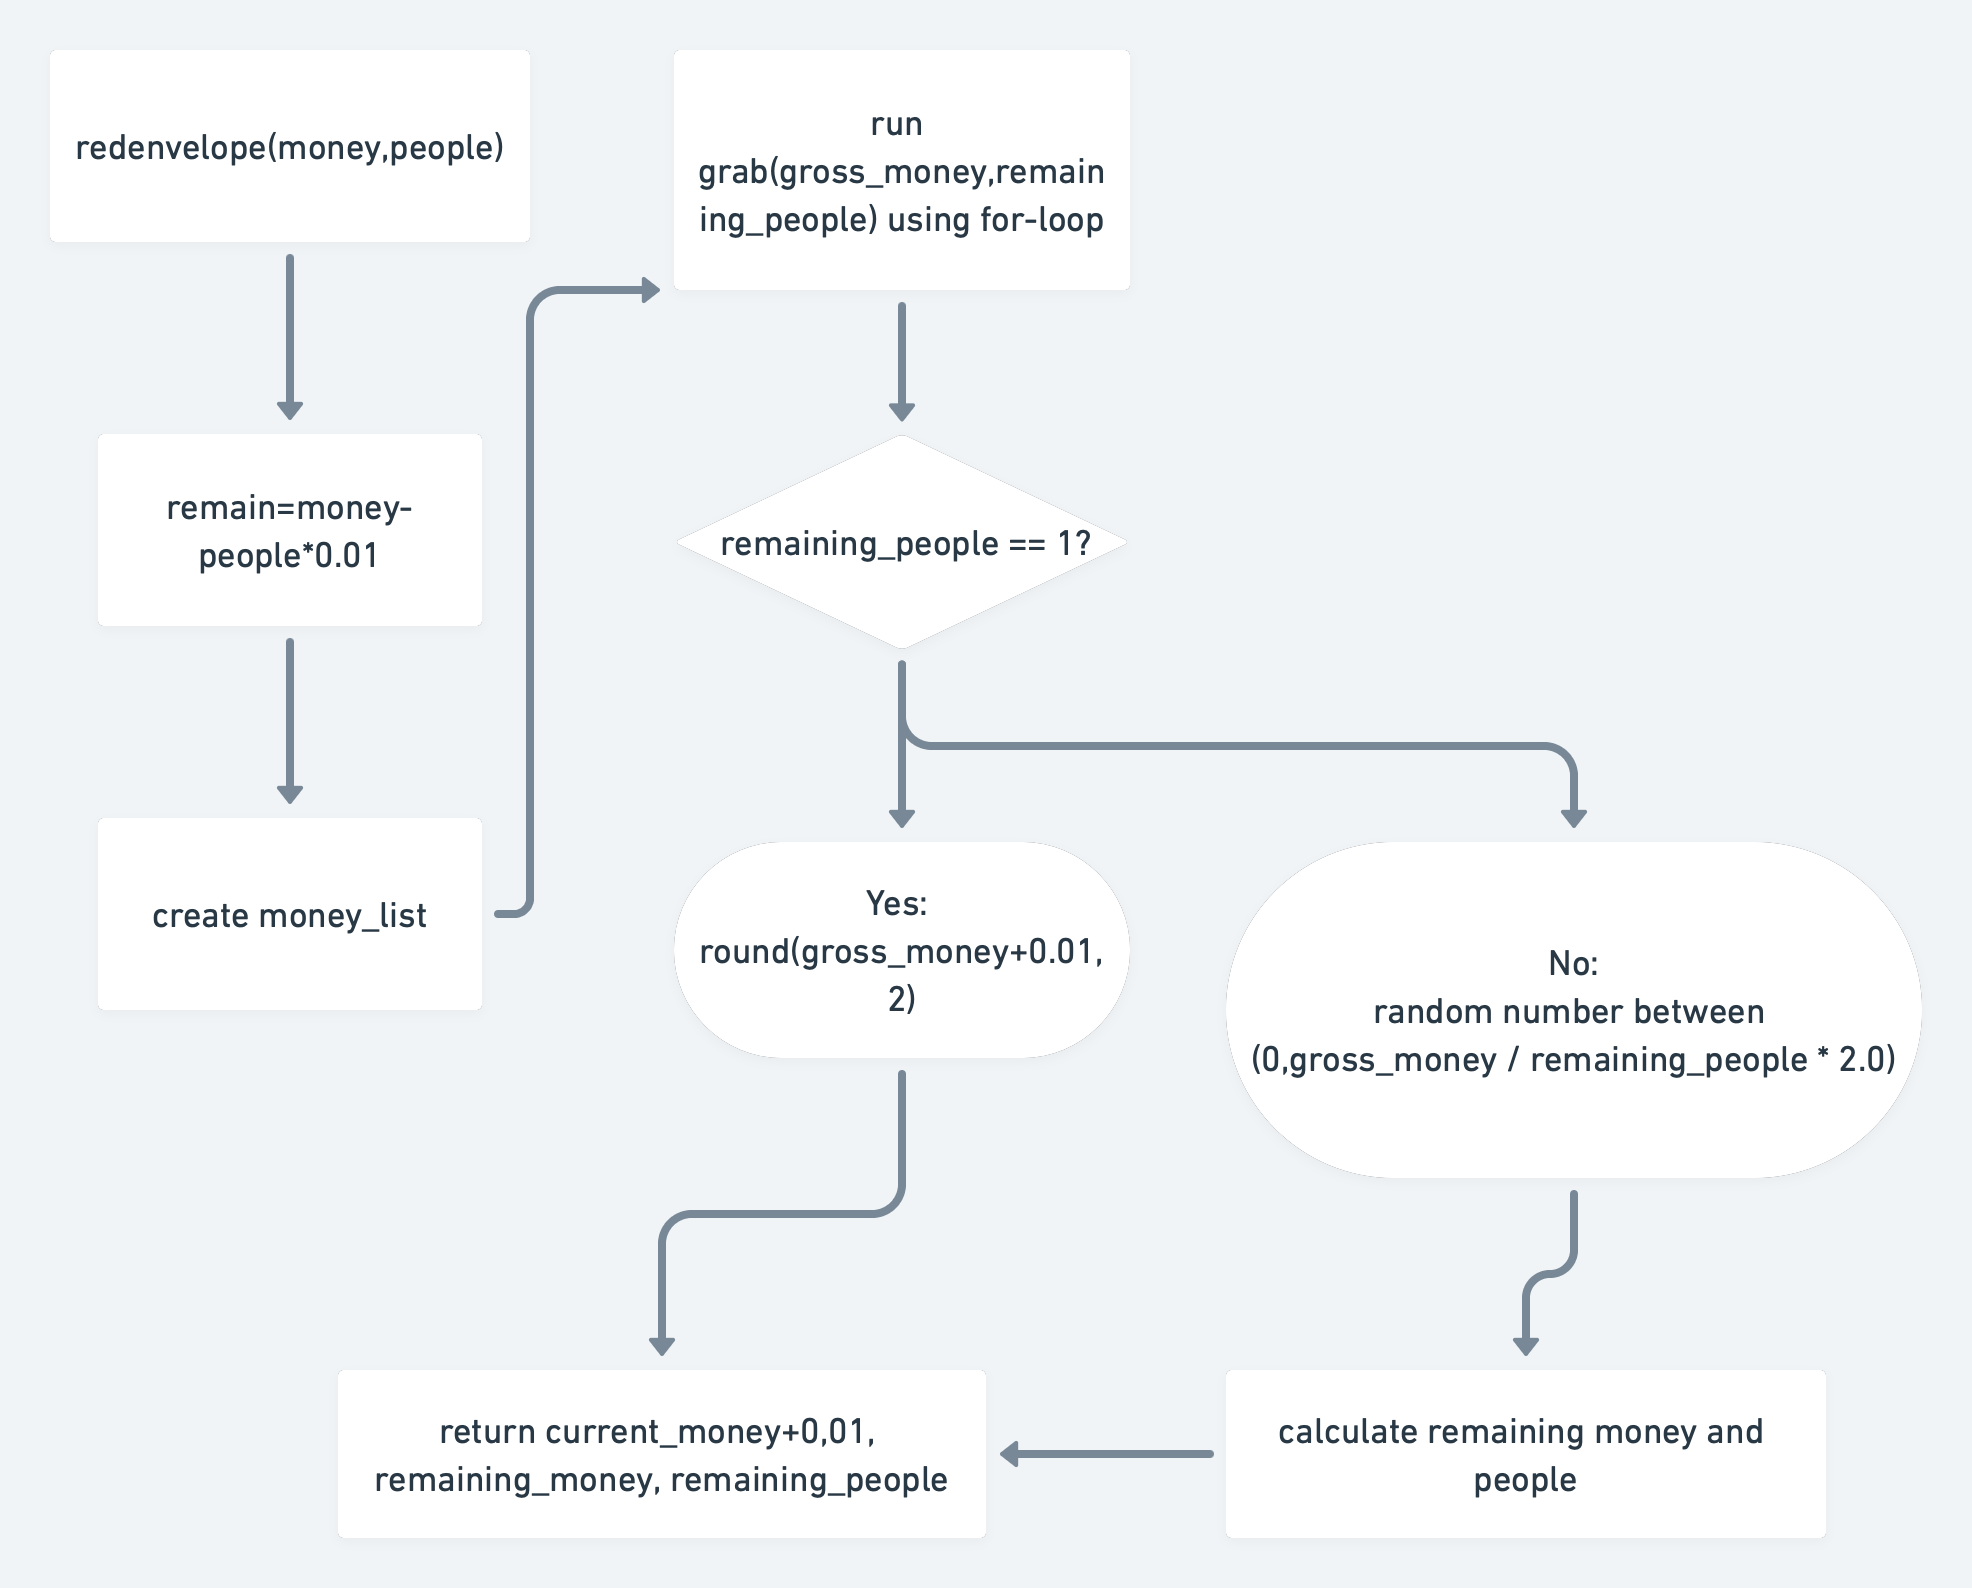
\includegraphics[width=15cm]{stats210@2x.png}
	\end{center}
	\caption{Basic Logic of the Main Function}
	\label{code}
\end{figure}


\section{Results}\label{sec4}
\subsection{Simulation Results and Comparison}\label{sec4.2}
The simulation is run on a 2020 MacBook Air with M1 chip and 16 GB memory. In total, 10000 simulations of 8 people grabbing 8 yuan's envelope are carried out.\footnote{The  CSV file of results can be downloaded at \url{www.yueqianlin.com/SimulatedResults.csv}.} We first try to compare our simulation results with the experimental results to validate our theory. As shown in Figure \ref{sca}, the results from the experiment and simulation have almost the same mean value, and they both did not exceed the theoretical boundary. In fact, as shown in Figure \ref{mean_var_sim}, the 10000 simulations show that the expectation of each order remains the same and the variance is increasing by order, which echoes our mathematical analysis in Section \ref{sec3.1}.
\begin{figure}[H]
	\begin{center}
		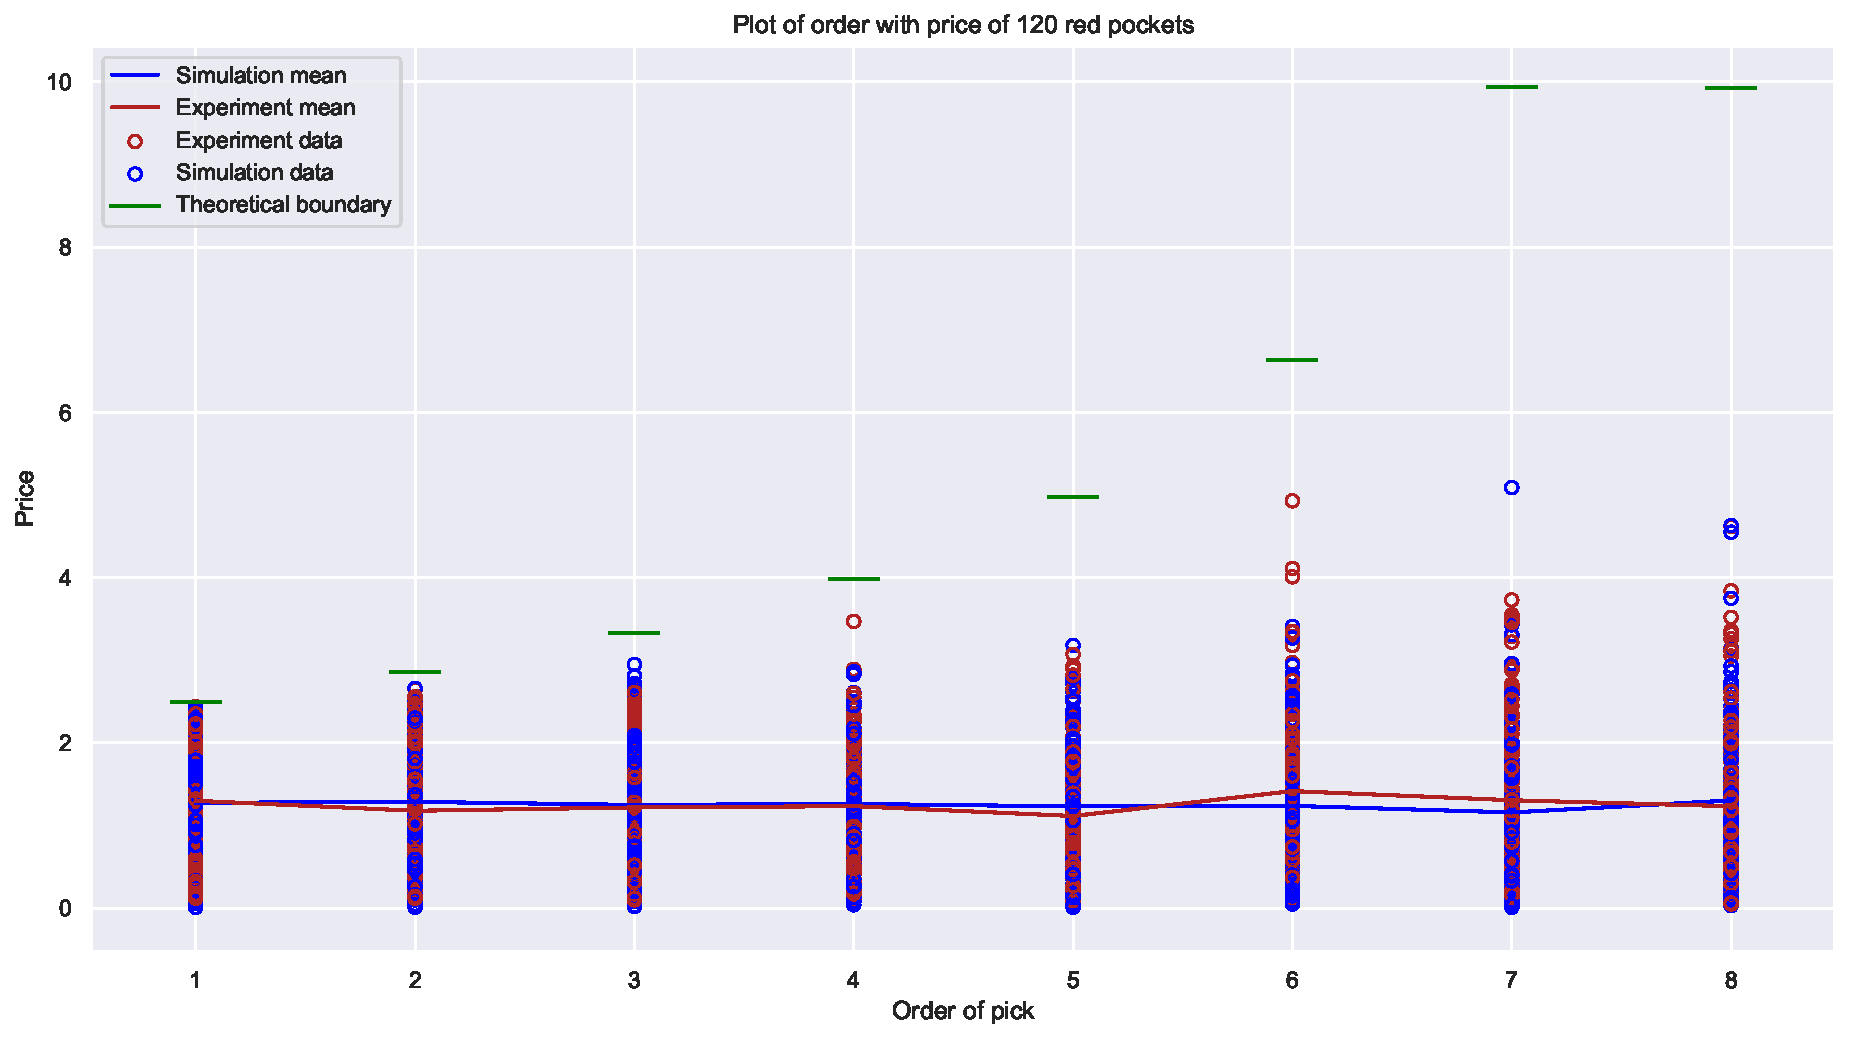
\includegraphics[width=16cm]{pic1.pdf}
	\end{center}
	\caption{Scatter Plot of Experiment and Simulation Results with Boundaries}
	\label{sca}
\end{figure}
\begin{figure}[H]
\centering    
\subfigure{
\label{mean_sim}
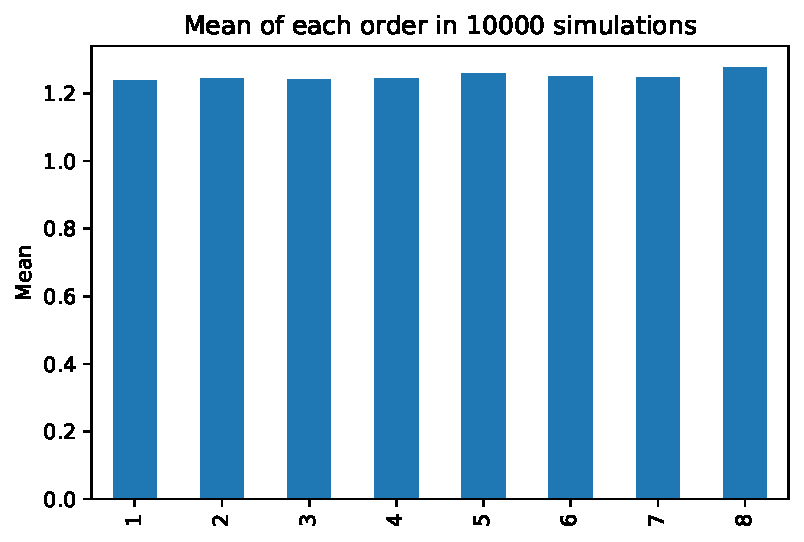
\includegraphics[width=0.4\columnwidth]{Mean of Each Order in 10000 Simulations.pdf}  
}     
\subfigure{ 
\label{var_sim}     
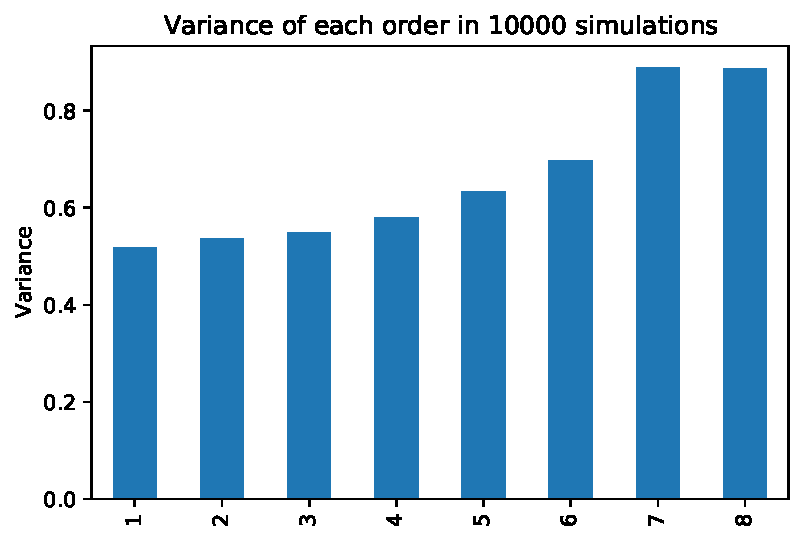
\includegraphics[width=0.4\columnwidth]{Variance of Each Order in Simulations.pdf}     
}    
\caption{ Mean and Variance of Each Order in 10000 Simulations}     
\label{mean_var_sim} 
\end{figure}
\par
To take a closer look of the money distribution in different grabbing order, the frequency distribution histograms of each pick's earned money in both simulation and experiment are plotted, as shown in Figure \ref{comp1}. Additionally, a 3-order polynomial function is used to approximate the money distribution in each order, and we calculate the correlation coefficients between the simulation function, which are quite high and indicate a strong correlation between our simulations and experiments.
\begin{figure}[H]
	\begin{center}
		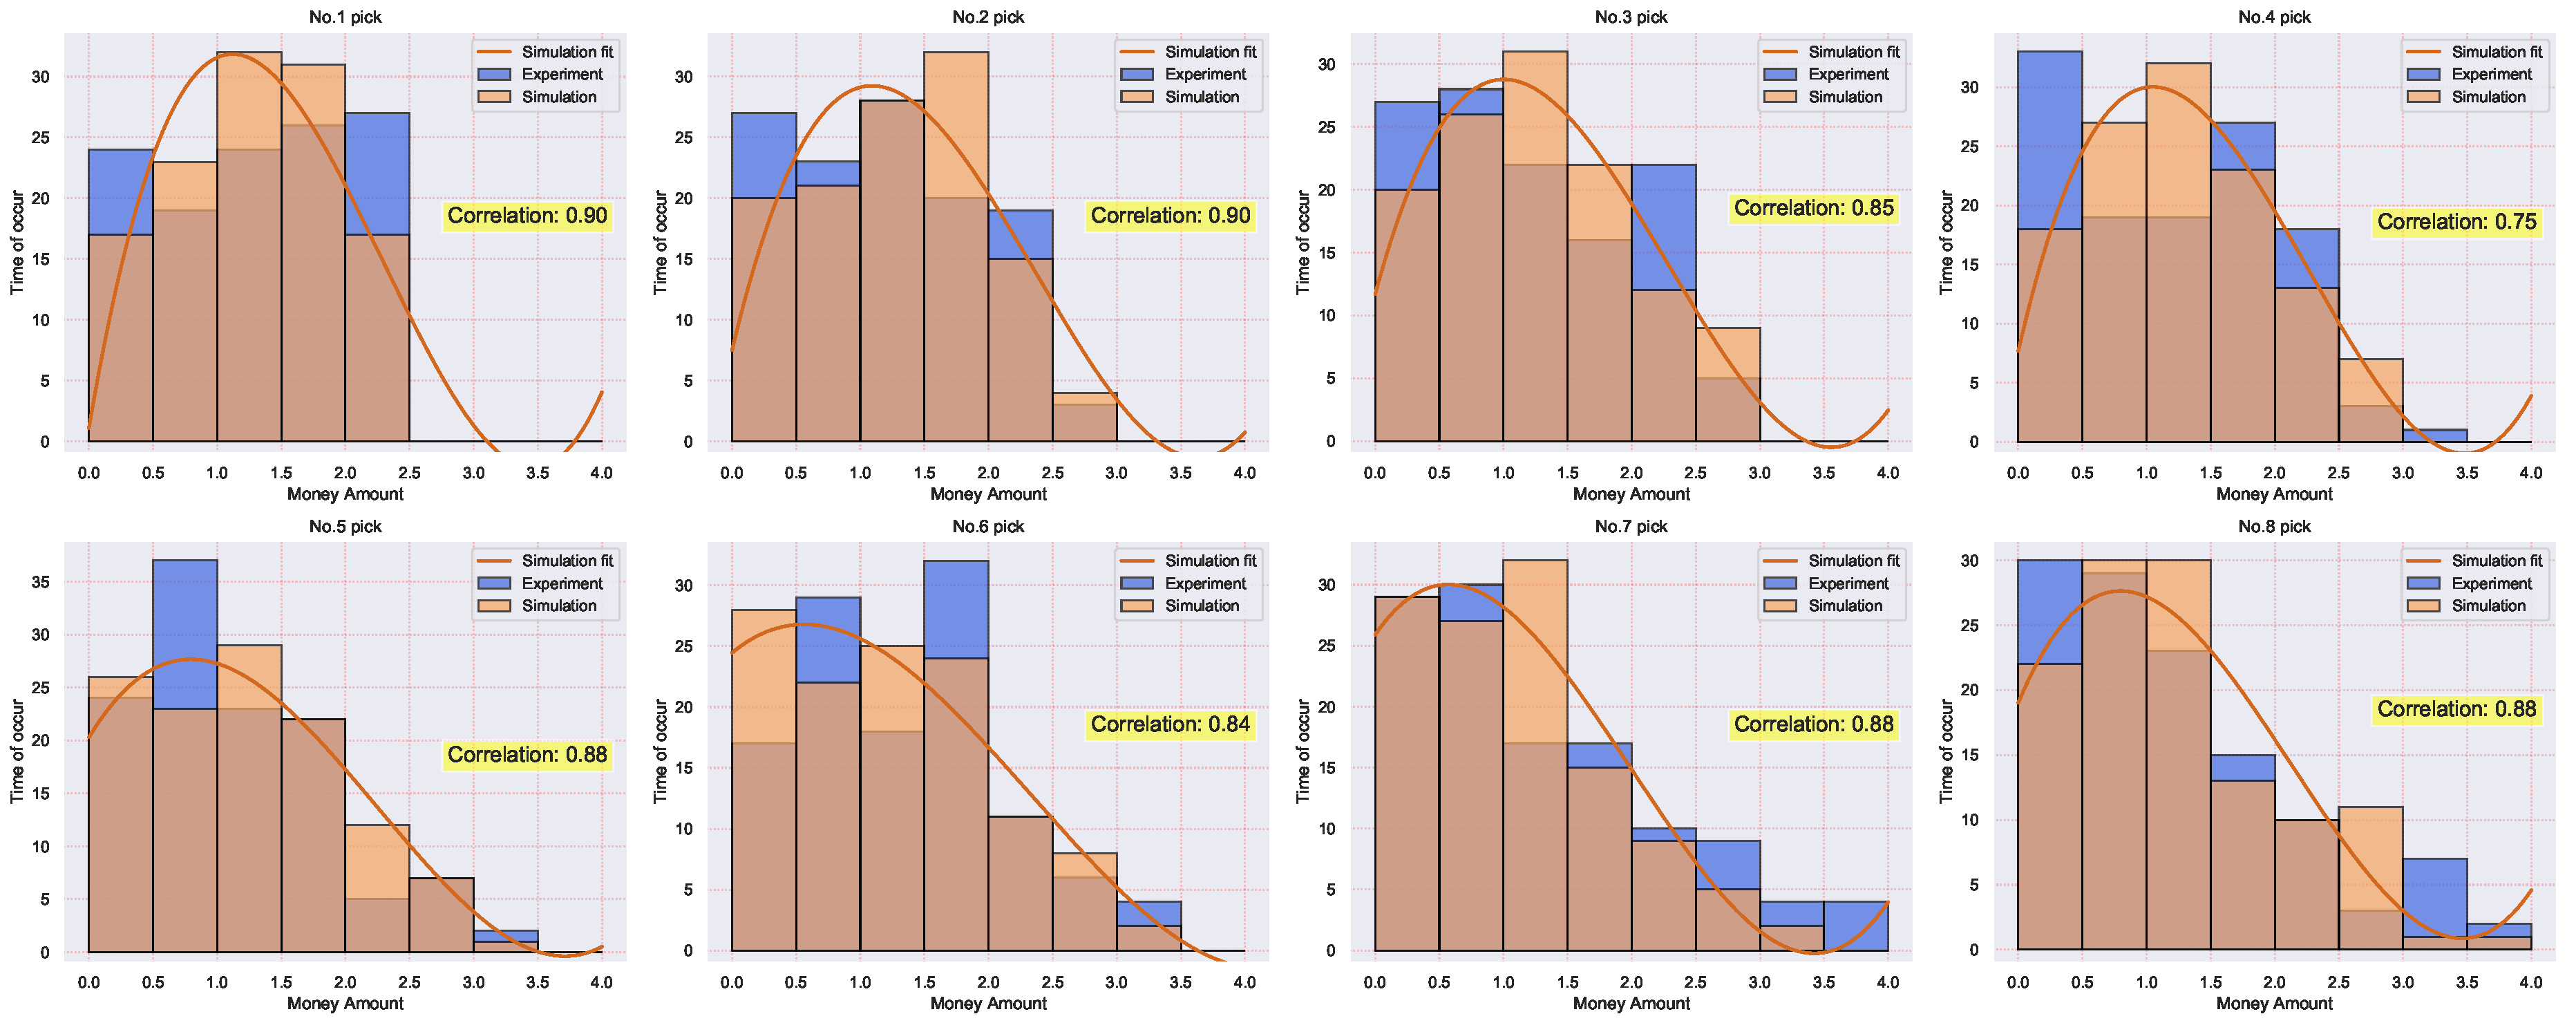
\includegraphics[width=16cm]{pic5.pdf}
	\end{center}
	\caption{Comparison between Simulation and Experiment Results}
	\label{comp1}
\end{figure}
\subsection{Suggestions}
For a WeChat random red envelope, statisitically speaking, the order of grabbing the red envelope does not significantly affect the amount of money grabbed, because the chances of grabbing the red envelope are equal. For a WeChat random red envelope, the only difference between different positions of grabbing the red envelope is the different fluctuation range of the random amount grabbed, and those who grab the red envelope first have a higher possibility of grabbing the average amount, while those who grab the red envelope later will either grab a smaller random amount or a larger random amount. Based on the risk preference structure, risk-avoiding people should try to grab red envelope earlier to guarantee a least amount of money. While risk-seeking people should grab later to have the opportunity of grabbing the biggest envelope.




\section{Additional Analysis}\label{sec5}
\subsection{Luckiest People in One Envelope}\label{sec5.1}
With the important theory we derive and validate, and with the simulation functions similar to the original WeChat envelope, many interesting analysis can be carried out.
First, we define the luckiest people in one envelope as the one grabbing the most money, and try to find the relation between the luckiest person and the order of grabbing. We find that people who grab at last will have the highest probability to receive the luckiest envelope, while in the mean time have the highest probability to receive the unluckiest envelope (Figure \ref{lucksim}). We divide the luckiest rate by the unluckiest rate and generate the luckiest/unluckiest rate, which indicates which order will have a relevant safer revenue. And it shows that the first one to grab the envelope is more likely to have a safer outcome, which also are similar to our previous analyis.\par


\begin{figure}[H]
\centering    
\subfigure{
\label{mean_sim}
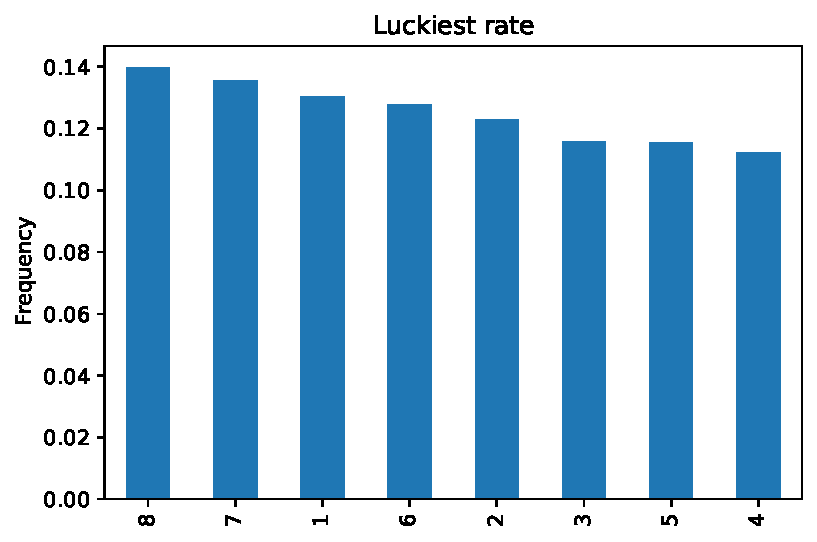
\includegraphics[width=0.3\columnwidth]{luckiest_rateOf10000Simulations(10-8).pdf}
}     
\subfigure{ 
\label{var_sim}     
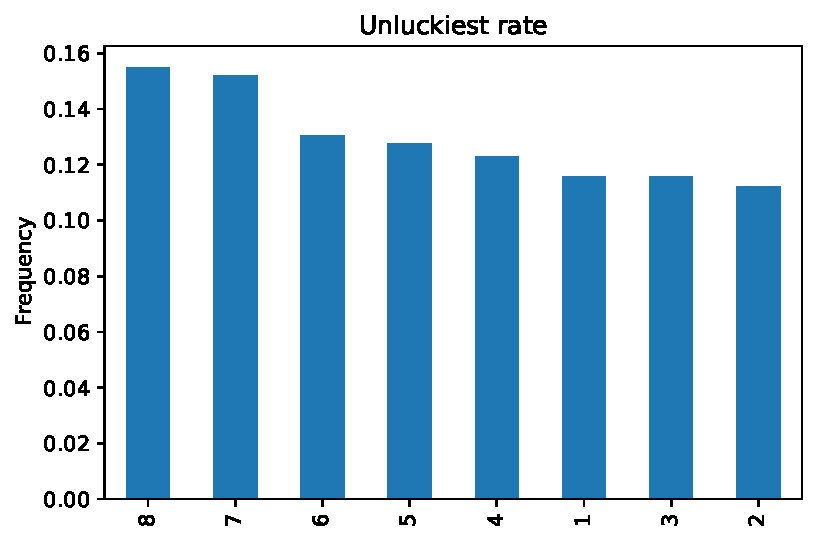
\includegraphics[width=0.3\columnwidth]{Unluckiest Rate of Each Order.pdf}     
}    
\subfigure{ 
\label{var_sim}     
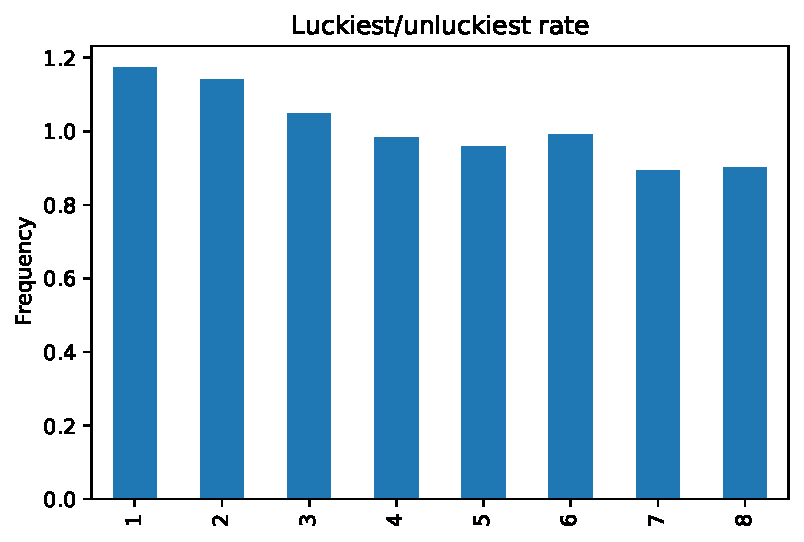
\includegraphics[width=0.3\columnwidth]{luckiest_unluckiest_rateOf10000Simulations.pdf}     
}  
\caption{Luckiest and Unluckiest Frequency in Different Order}     
\label{lucksim} 
\end{figure}
\par
Now, we extend this problem to more people grabbing the same envelope and want to find a more general pattern. We carry out 10000 simulations of 3 to 14 people grabbing 10 yuan. As shown in Figure \ref{box}, the results are parallel to our theoretical analysis: the expectation of each envelope is almost the same ($\frac{\text{Money}}{\text{Overall People}}$), and the variance is increasing by order while the last two orders' variance are almost the same. Then, back to the luckiest people topic, we find out that the distribution is not exactly change in scale when the amount of people is increasing. Figure \ref{luck3} shows the distributions, where from 3 to 6 people, the luckiest people seems to be the first one to grab the envelope, and from 7 to 14 people, the luckiest people become one of the last two people. Also, it seems to become a "U" shape where the 
right end is increasing as the amount of people increases. More rigorous proof may be needed to for this finding. However, if one would like to be or avoid being a luckiest people in one envelope, he/she could refer to the finding above.
\begin{figure}[H]
	\begin{center}
		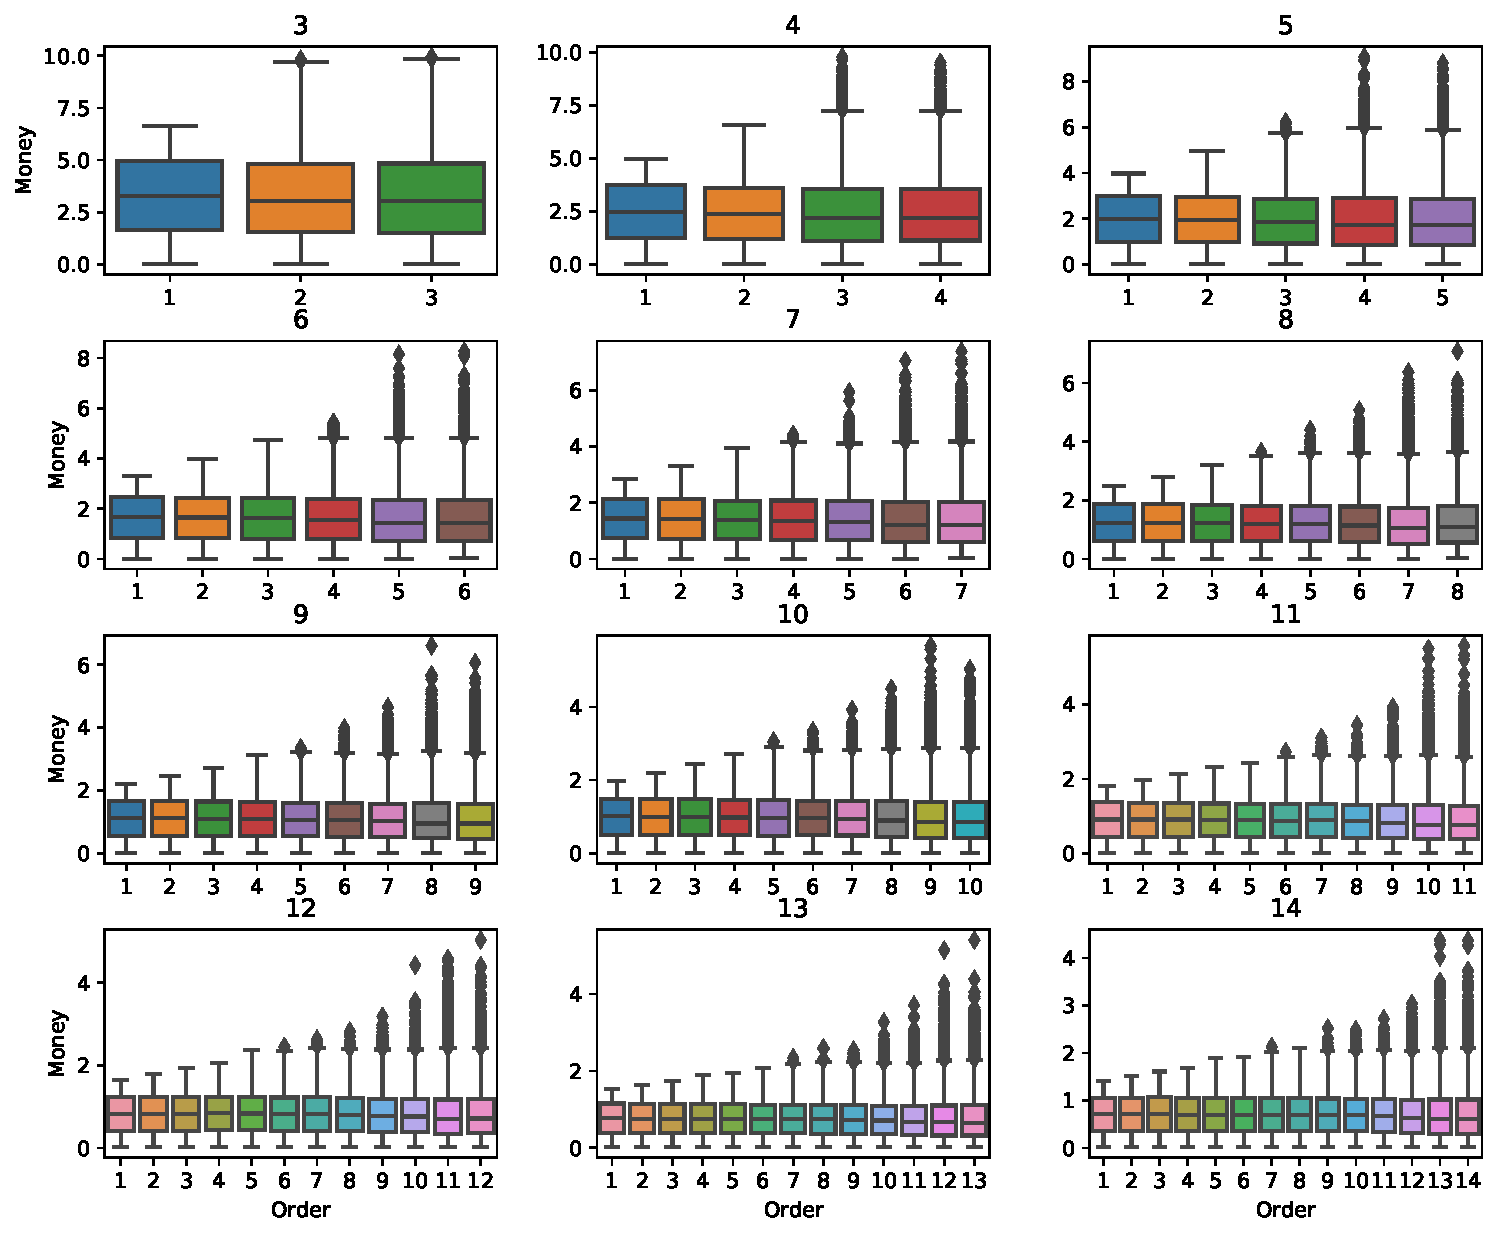
\includegraphics[width=16cm]{boxplot_3-14people10000simulation.pdf}
	\end{center}
	\caption{Box Plot of 3-14 People Envelope in 10000 Simulations}
	\label{box}
\end{figure}
\begin{figure}[H]
	\begin{center}
		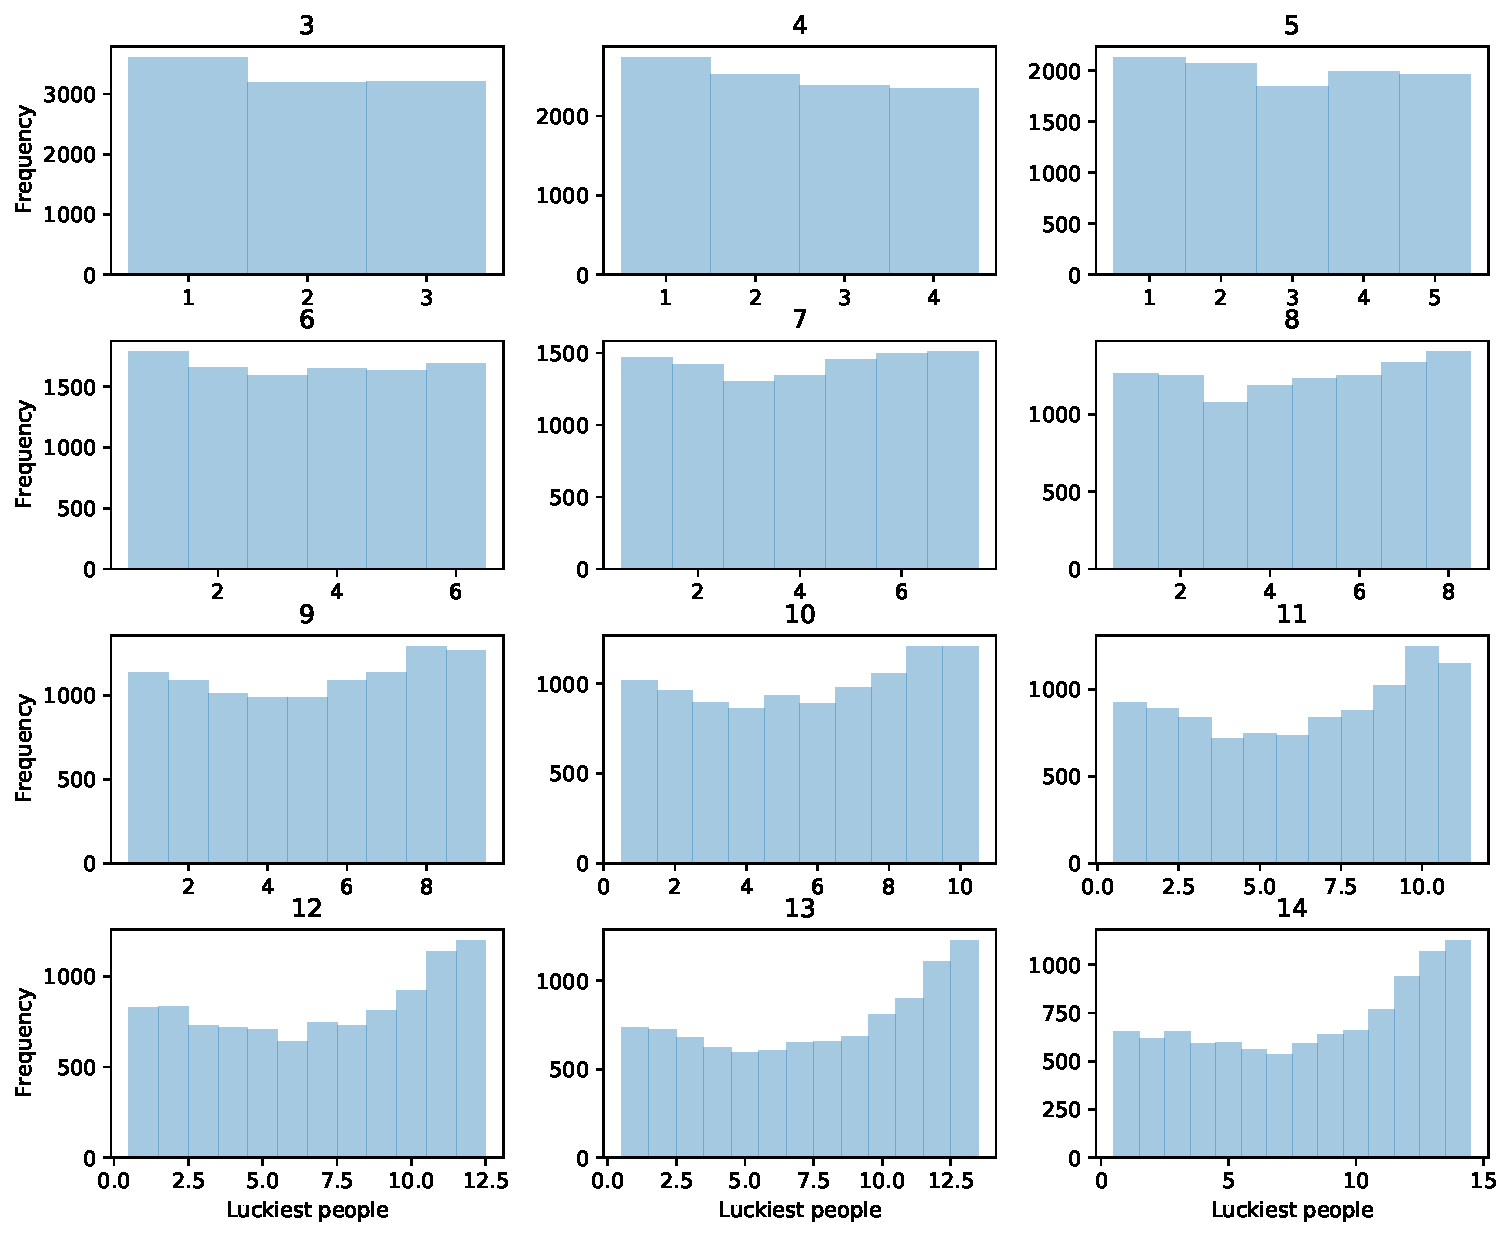
\includegraphics[width=16cm]{luckiest3-14people10000simulation.pdf}
	\end{center}
	\caption{Luckiest Pick among 3-14 People in 100000 Simulations  }
	\label{luck3}
\end{figure}
\subsection{Red Envelope Solitaire}
One of the reasons behind our analysis on the luckiest people in Section \ref{sec6} is that there is a trend in China that whoever grab most money should continue to give others' red envelopes, just as solitaries. We simplify the problem and discuss the following two scenarios: with 8 people and 10 yuan in each round 1) people will grab in a fixed order; 2) people will grab in a random order.\footnote{The simulation codes are listed in Appendix \ref{appendix2}.} In total 10000 trails are carried out where each trial has 100 rounds of red envelope. The box plot of the mean of the 100 rounds in 10000 simulation results can be found in Figure \ref{luckgamesim}. For a fixed grabbing order, the ones who choose to grab the envelope in the middle will most likely to be profitable. While in a random order of grabbing, it seem that only the first people who send out the red envelope initially will lose money, and the other people will have similar profits. The second scenario may be more realistic and it seem that people who send out the envelope at fist will lose the money.

\begin{figure}[H]
\centering    
\subfigure{
\label{1}
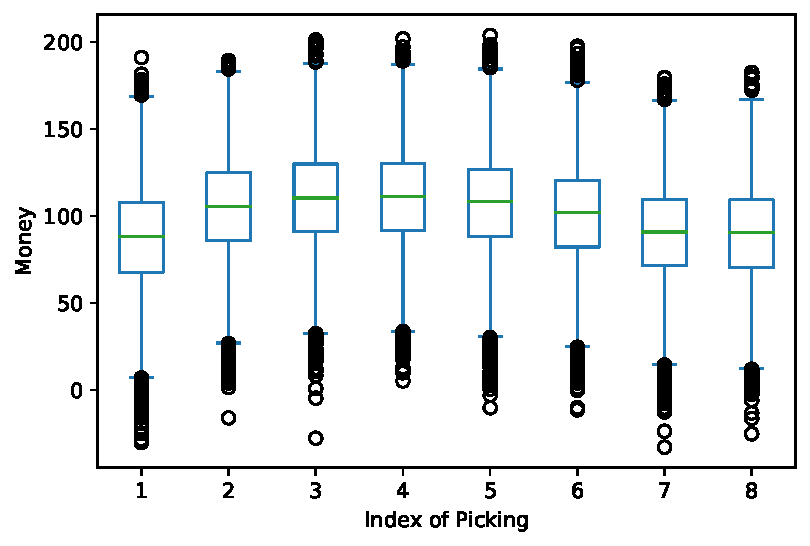
\includegraphics[width=0.4\columnwidth]{fixed_picking.pdf}
}     
\subfigure{ 
\label{2}
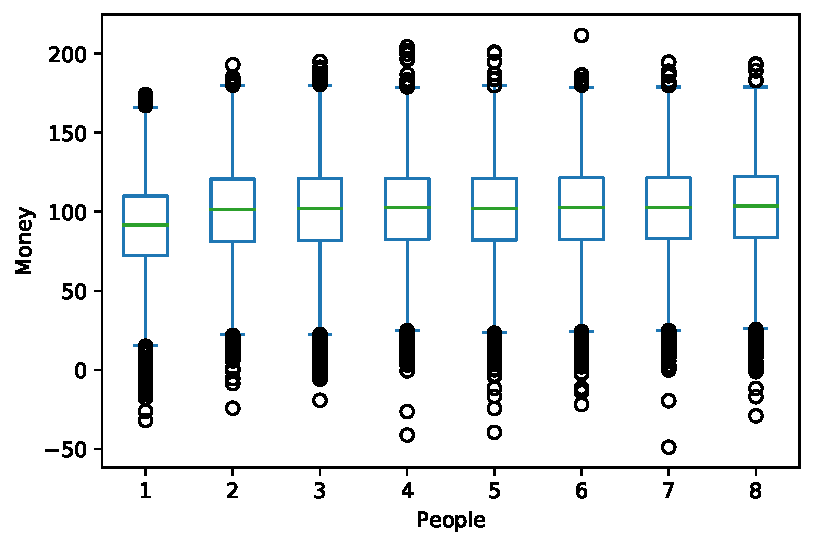
\includegraphics[width=0.4\columnwidth]{random_picking.pdf}     
}
\caption{Fixed and Random Oder Grabbing in the Solitaire}
\label{luckgamesim} 
\end{figure}
\subsection{Red Envelop Rain}
Another thing we want to achieve is to actually apply our knowledge and create our own version of sending and receiving red envelopes. However, this requires many software and web development s kills and we have to abandon the idea at last. However, we do have a demo version of the Red Envelope which is not perfect and has a bad randomized results \cite{byzantine-pki}.\footnote{The demo version of the Red Envelope Rain can be found at \url{www.yueqianlin.com/red_envelope}.}. We hope we can learn more useful knowledge in the near future and refine this project.
\section{Conclusion}
\label{sec6}
Wechat random red envelope is a common random process in our daily life. Through the experiment of asking 8 people to grab 120 red envelopes on WeChat, we get the result that the expected value of the grabbed amount does not change with the order of grabbing. However, we found that late grabbers were more likely to grab both the maximum and minimum amount of money. Then, we establish a theory to explain this, which is based on the nature that the previous quantity will have an impact on future process. We can mathematically prove that $\operatorname{Var} X_{1}<\operatorname{Var} X_{2}<\ldots<\operatorname{Var} X_{n-1} = \operatorname{Var} X_{n}$.\par
This means that as the red packet is grabbed, the variation in the amount will increase, and it will peak at the last two grabbers. Based on this theory, we implement our simulation model in Python and verify our simulation results with experimental results, which shows that our model is effective. Summarizing all our findings in experiments, modeling and simulation, the strategies to obtain more money from WeChat red envelopes are as follows. If there are a small number of participants (3-8), and the number of red envelops is very limited, then grabbing as soon as possible will maximize the benefits since you may get nothing if you grab too late. If there are a large number of participants (8 or more), there are two strategies: the safe method is to grab as soon as possible, and the risk choice is to wait until the end to try to grab the last two packets, which are likely to be super large or super small. However, when the number of red envelopes is very large, the amount of money received by each grabber will eventually converge to the average as expectation. Additional analysis is made for luckiest people solitaire game strategy.

\section*{Author Contributions}
YL wrote the Python simulation code and drew the plots. He was responsible for writing Section \ref{sec3.3}, \ref{sec4} and \ref{sec5}. JH was responsible for writing Section
\ref{sec1}, \ref{sec2.1}, \ref{sec3.1} and \ref{sec6}. ZZ was responsible for drawing plots and writing Section \ref{sec2.2}. XZ was responsible for designing the distribution mechanism, and writing Section \ref{sec1} and \ref{sec3.1}.
\newpage
\singlespacing
\bibliographystyle{IEEEtran}

\bibliography{references}

\printbibliography{}
\newpage

%------ To create Appendix with additional stuff -------%
%\newpage
% \addcontentsline{toc}{section}{Appendix}
\appendix
\section{Appendix}\label{appendix1}
\subsection{Main Function}
\begin{lstlisting}[language = Python,title={main.py},  numbers=left, 
    numberstyle=\tiny,keywordstyle=\color{blue!70},
    commentstyle=\color{red!50!green!50!blue!50},frame=shadowbox,
    rulesepcolor=\color{red!20!green!20!blue!20},basicstyle=\ttfamily]
import random
import math
def redenvelope(money,people):
  # make sure all people have at least 0.01 yuan
  remain = money - people * 0.01
  remaining_people=people
  money_list=[]
  for i in range(people):
    [current,remain,remaining_people]=grab(remain,remaining_people)
    money_list.append(current)
  return money_list
def grab(gross_money,remaining_people):
  if remaining_people == 1:
    return round(gross_money+0.01,2),0,0
  min_value = 0.0
  max_value = gross_money / remaining_people * 2.0
  current = random.random() * max_value
  current= min_value if current < min_value else current
  current=math.floor(current * 100) / 100.0
  remain = round((gross_money - current),2)
  remain=gross_money-current
  return round(current+0.01,2),remain,remaining_people-1
\end{lstlisting}
\subsection{Solitaire Code}\label{appendix2}
\begin{lstlisting}[language = Python,title={solitaire.py},  numbers=left, 
    numberstyle=\tiny,keywordstyle=\color{blue!70},
    commentstyle=\color{red!50!green!50!blue!50},frame=shadowbox,
    rulesepcolor=\color{red!20!green!20!blue!20},basicstyle=\ttfamily]
import pandas as pd
import random
df=pd.DataFrame(columns=range(1,8+1))
for k in range(10000):
    money_list=np.array([100 for i in range(8)])
    luck=0
    record=[]
    record_trial=[]
    for i in range(100):
        money_list[luck]-=10
        t=redenvelope(10,8)
        # remove the # mark in the following line if 
        # want to use random order
        # random.shuffle(t)
        t=np.array(t).astype(float)
        luck=t.argmax()
        money_list=money_list+t
    df.loc[k]=money_list
\end{lstlisting}
%Put data files, CAD drawings, additional sketches, etc.

\end{document}
